\chapter{Implementation - "Building the solution"}


\section{Introduction}

This chapter is a walkthrough of the steps which describe the construction of the application.

\section{Terminal}

\subsection{Command Line Instructions}

As this application was centred towards security and being secure as the data it would hold would need to be kept safe. Therefore it made sense to focus on a good login with authentication and authorisation. To start working with Symfony, one needs to setup the Symfony environment through an installation process before Symfony applications can be created. Instructions for this can be found on the SensioLabs Symfony website. Navigating to the Documentation page. In there can be found Chapter 1 which has the Setup instructions under the Get Started dropdown menu. They explain the different ways for installing and setting up the Symfony framework for both Mac OS and Windows. Along with some\newline troubleshooting ideas if there are any problems with the installation. This application was built on a Mac OS so the instructions would vary slightly due to the command line instructions used. Using the installer made it easy to create this application with Symfony and only needed to be done once as it was installed globally on the machine.

\begin{figure}[htbp]
   \centering
   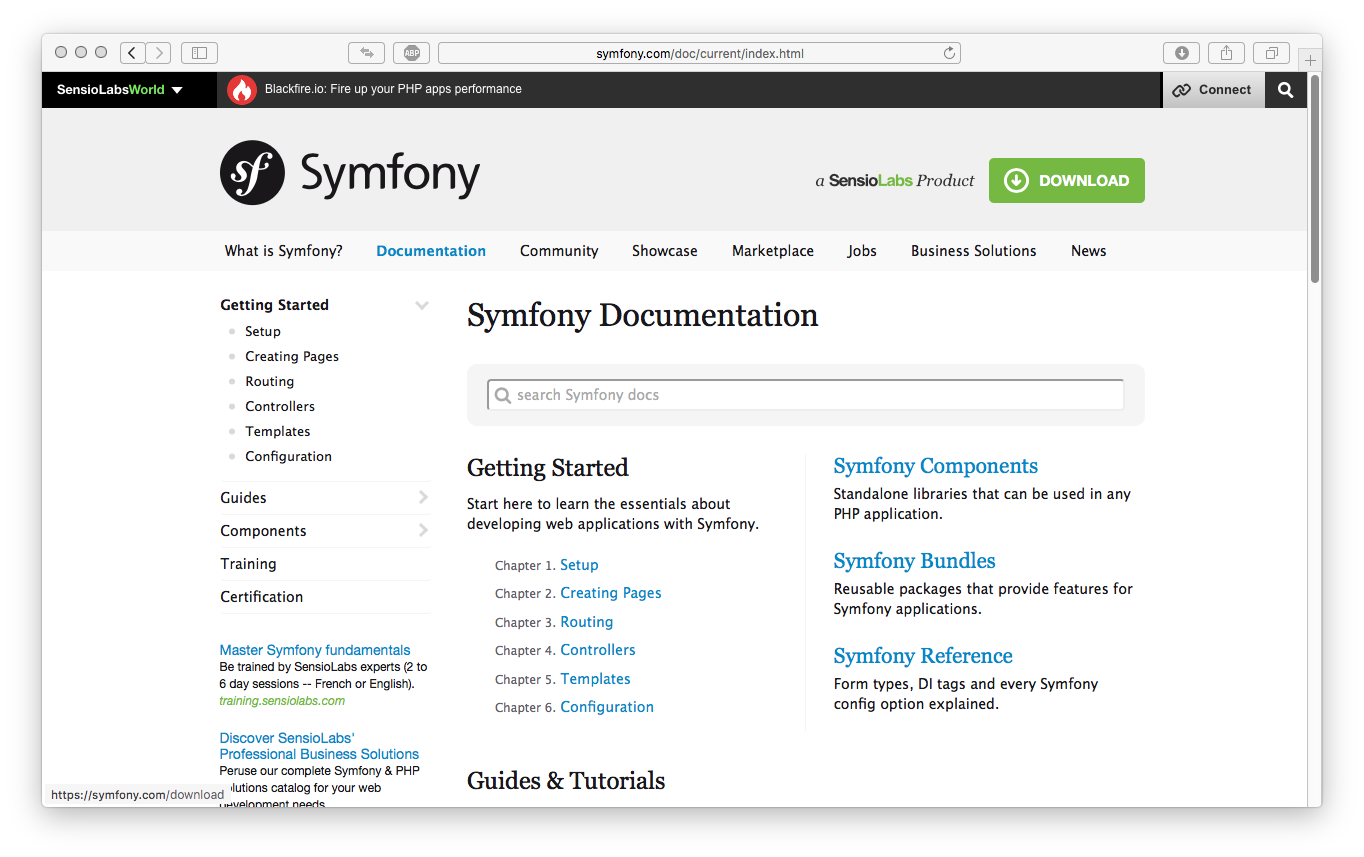
\includegraphics[width=400pt]{figures/symfony_documentation.png} % requires the graphicx package
   \caption{Symfony Documentation}
   \label{fig:Symfony Documentation}
\end{figure}

\begin{figure}[htbp]
   \centering
   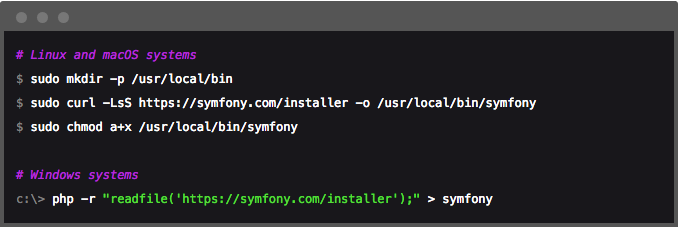
\includegraphics[width=400pt]{figures/symfony_installation.png} % requires the graphicx package
   \caption{Symfony Installation Setup}
   \label{fig:Symfony Installation Setup}
\end{figure}

With this completed moving into the directory or environment that the application will live which was the desktop. A final command in the terminal window was issued. This time starting with symfony new and by giving a project a name of choice thereafter. In this case the name COMPH4021-Project was used. The project was based on the current version of Symfony which is version 3.2.8. However, other versions can be specified after the project name in the terminal window. Once this part was completed. All required components were downloaded into a project folder with the name of which was given. The components are a set of files and directories which form the web application which use the Symfony libraries. The installer also carries out a check to make sure all requirements are met. If requirements are not all met a list is generated which provides the changes that are needed. In this case no changes needed to be made.

\begin{figure}[htbp]
   \centering
   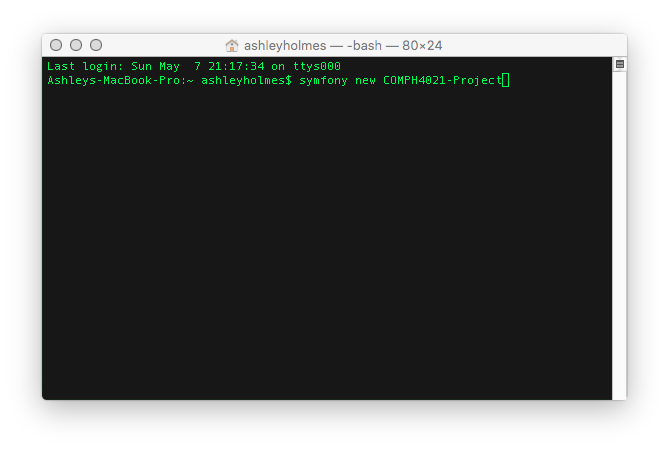
\includegraphics[width=400pt]{figures/new_application.png} % requires the graphicx package
   \caption{Symfony Application Setup}
   \label{fig:Symfony Application Setup}
\end{figure}

The below figure \ref{fig:Terminal Window Top} displays the command issued to download the project folder and following that in figure \ref{fig:Terminal Window Bottom} one can see that the project is being prepared and where it will be stored. In this case it was stored in /Users/ashleyholmes/Desktop/COMPH4021-Project.

\begin{figure}[htbp]
   \centering
   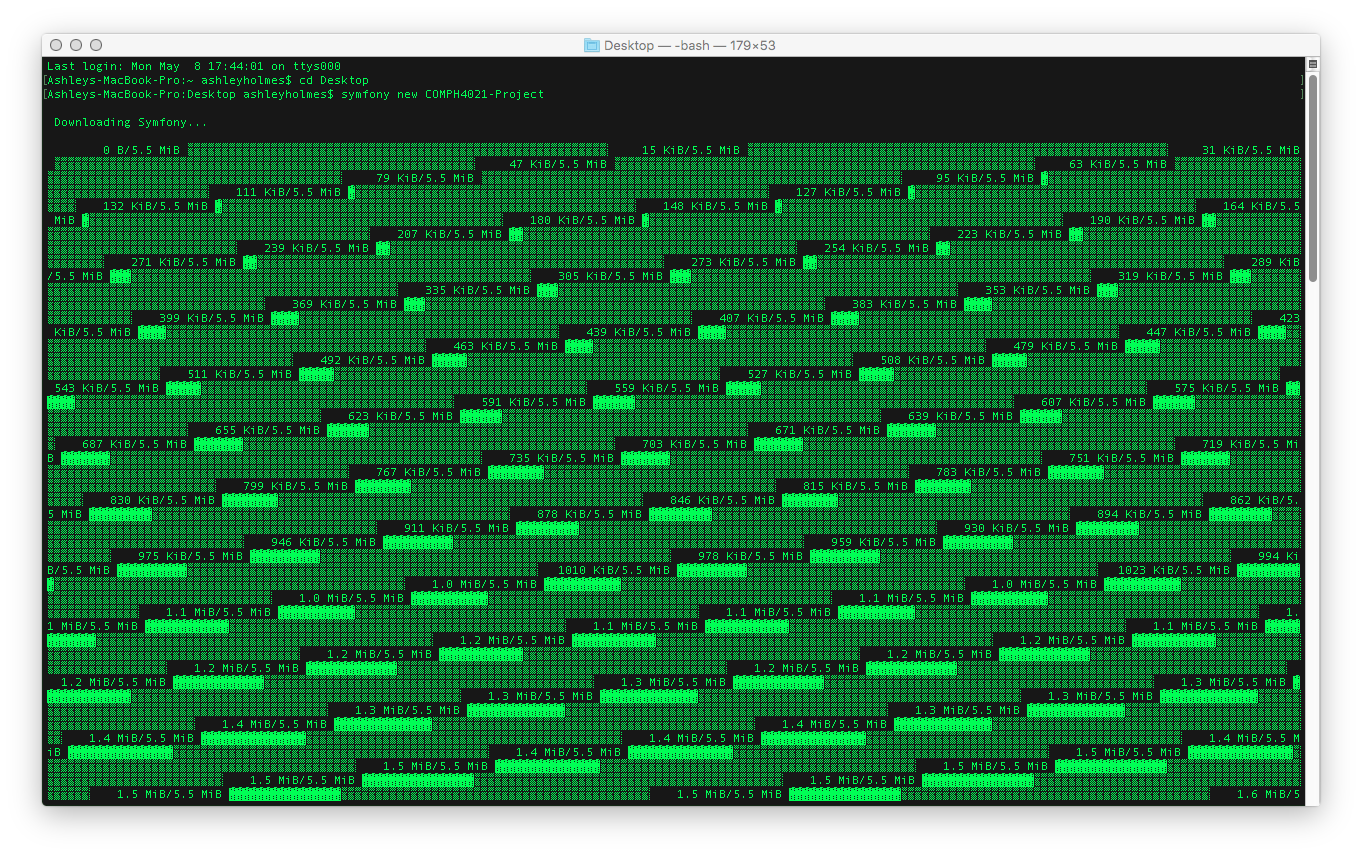
\includegraphics[width=400pt]{figures/terminal_window_top.png} % requires the graphicx package
   \caption{Terminal Window Top}
   \label{fig:Terminal Window Top}
\end{figure}

\begin{figure}[htbp]
   \centering
   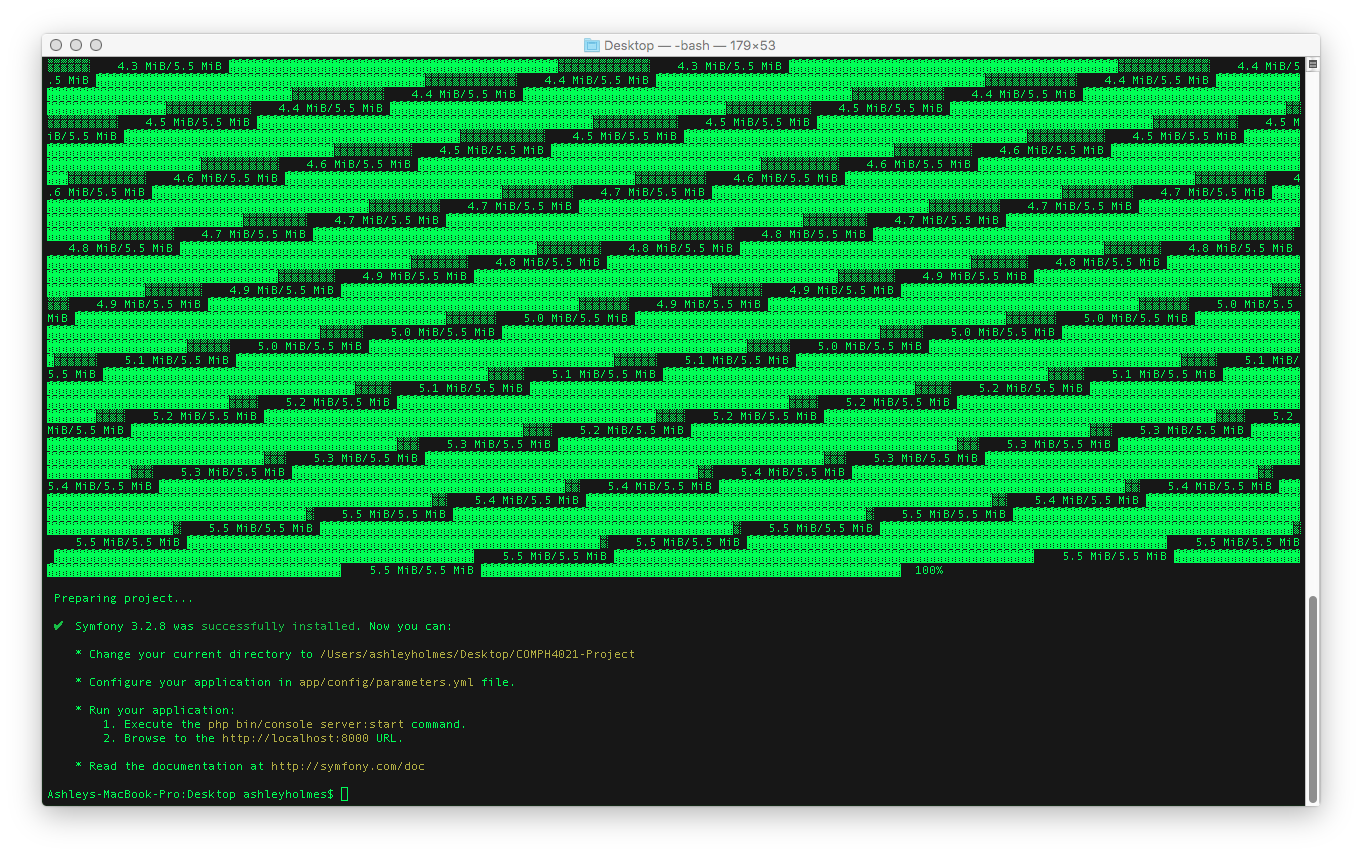
\includegraphics[width=400pt]{figures/terminal_window_bottom.png} % requires the graphicx package
   \caption{Terminal Window Bottom}
   \label{fig:Terminal Window Bottom}
\end{figure}

\begin{figure}[htbp]
   \centering
   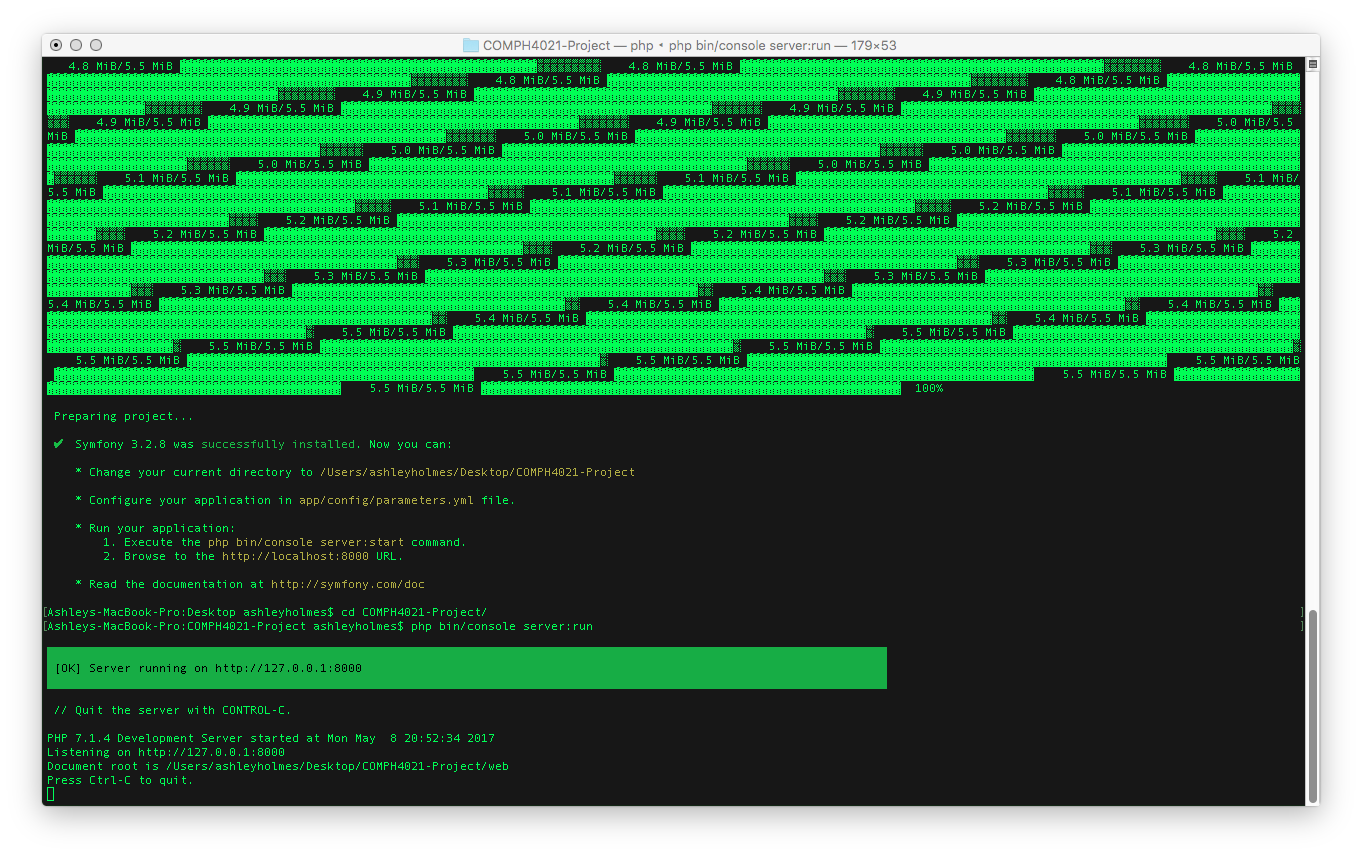
\includegraphics[width=400pt]{figures/php_server_run.png} % requires the graphicx package
   \caption{Php Server Run}
   \label{fig:Php Server Run}
\end{figure}

\begin{figure}[htbp]
   \centering
   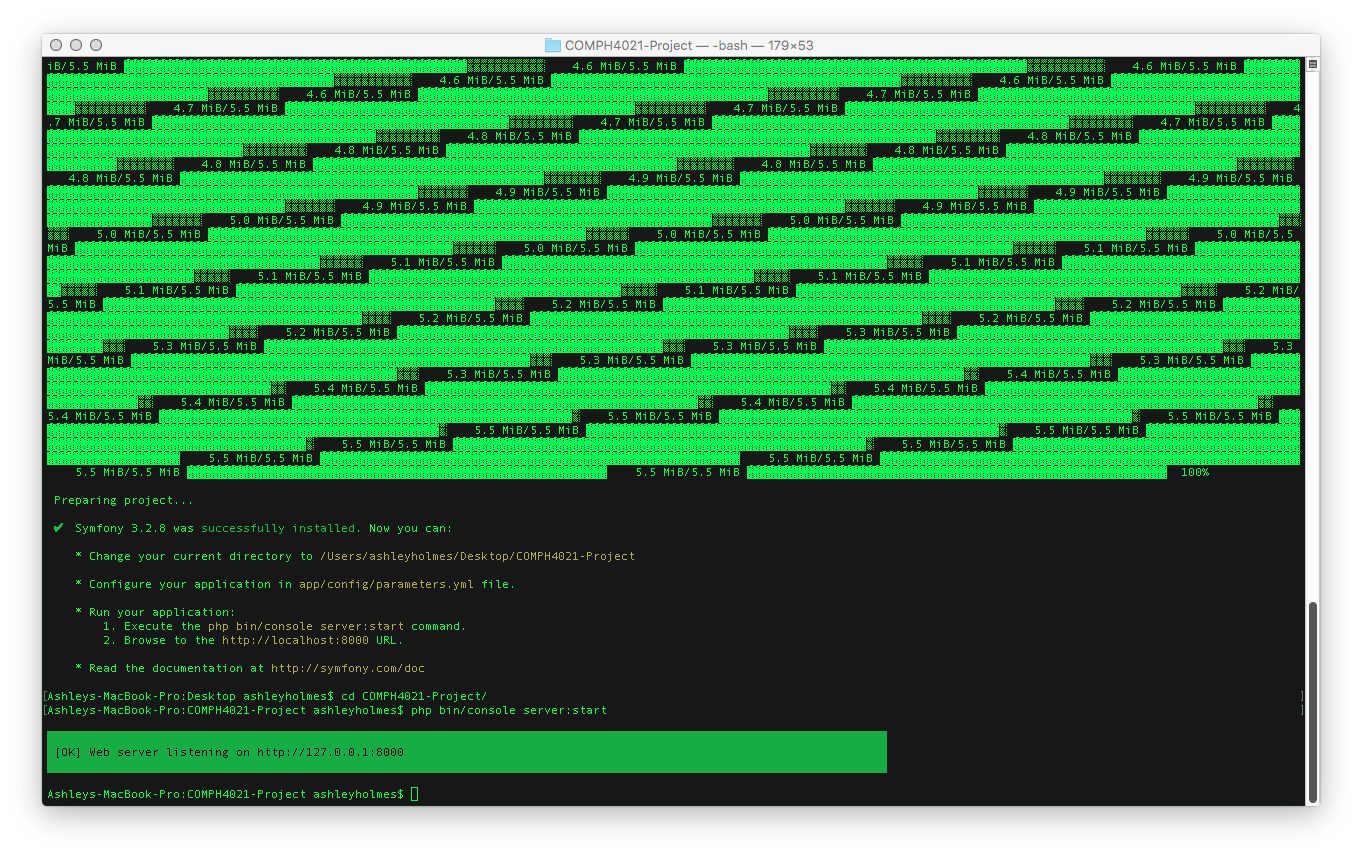
\includegraphics[width=400pt]{figures/php_server_start.png} % requires the graphicx package
   \caption{Php Server Start}
   \label{fig:Php Server Start}
\end{figure}

The next step would be to change directory into the COMPH4021-Project directory as this is where the built in Php server needs to be run from. NGINX and Apache may be used as alternatives however, since the Php server is built in. It makes development much easier. Executing the following command php bin/console server:run starts the server. However, once issuing this command the open terminal window would now need to remain out of use while the server is running. One can use a separate terminal window or open a new tab to issue any addition commands which are needed or make use of the PhpStorm terminal window. To run other processes in the background, issuing a php bin/console server:start will make it possible to execute commands in the same window which was done here. The difference can be seen in figure \ref{fig:Php Server Run} and figure \ref{fig:Php Server Start}.

\section{Browser}

\subsection{Deploying the Application}

\begin{figure}[htbp]
   \centering
   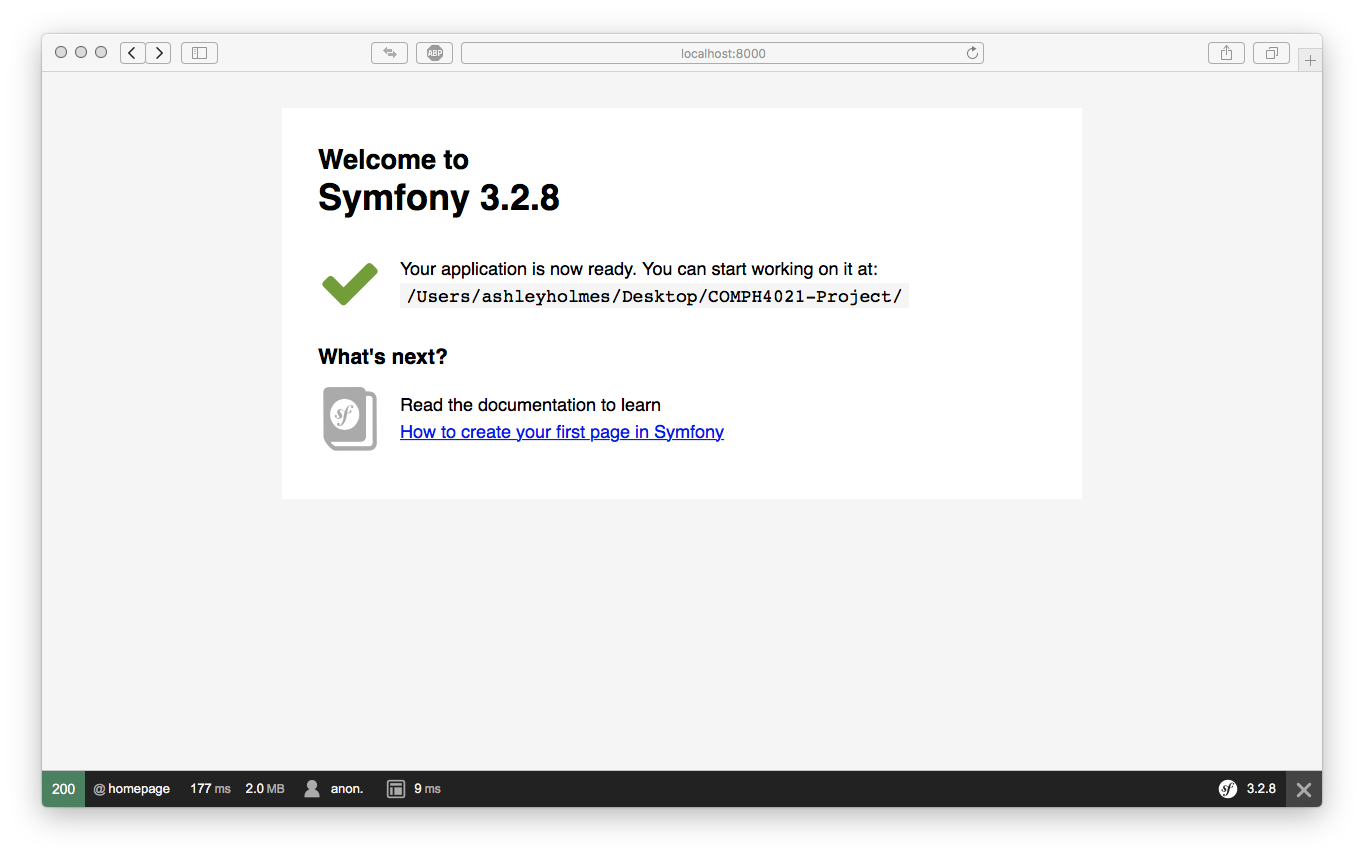
\includegraphics[width=400pt]{figures/symfony_browser.png} % requires the graphicx package
   \caption{Symfony Browser}
   \label{fig:Symfony Browser}
\end{figure}

\begin{figure}[htbp]
   \centering
   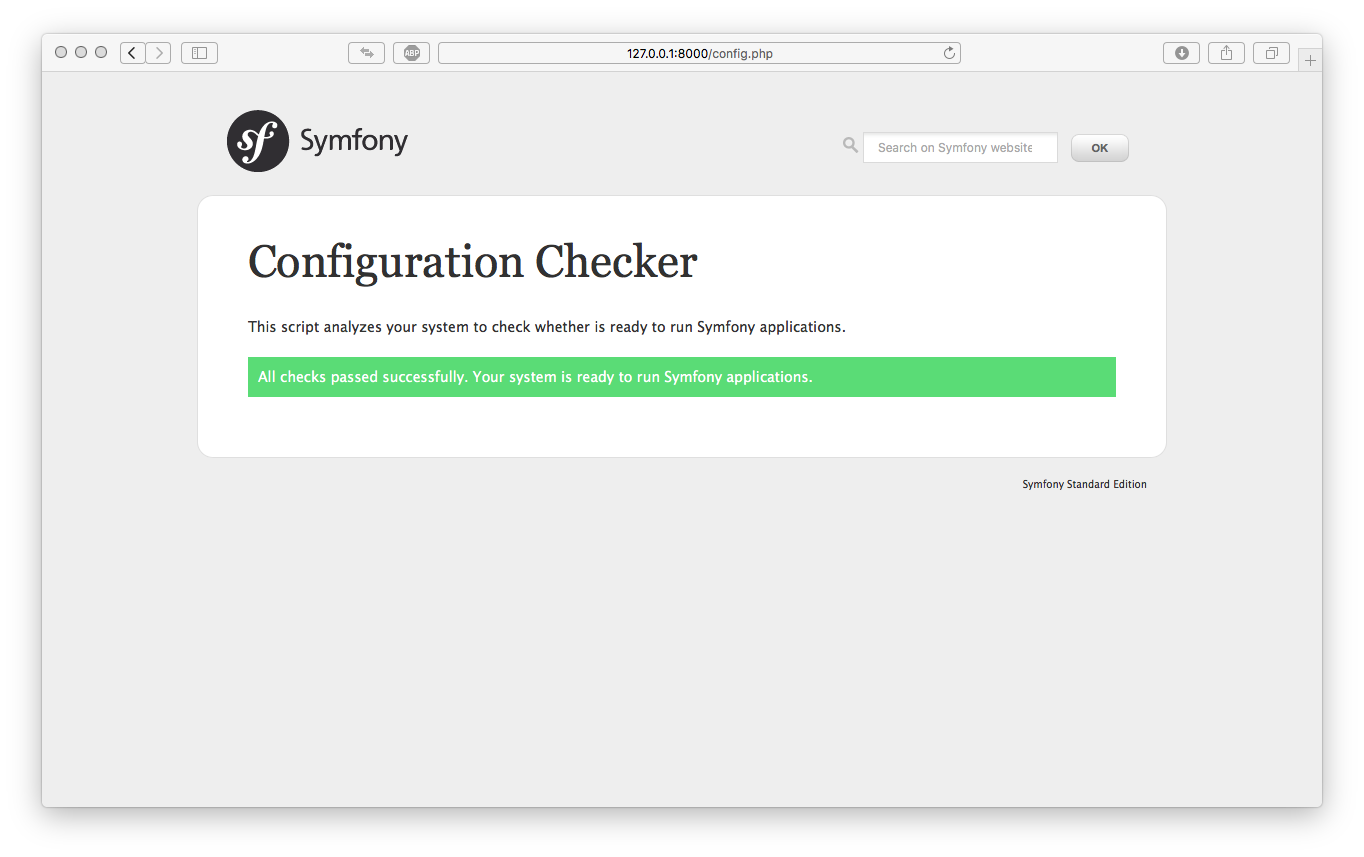
\includegraphics[width=400pt]{figures/configuration_checker.png} % requires the graphicx package
   \caption{Configuration Checker}
   \label{fig:Configuration Checker}
\end{figure}

\begin{figure}[htbp]
   \centering
   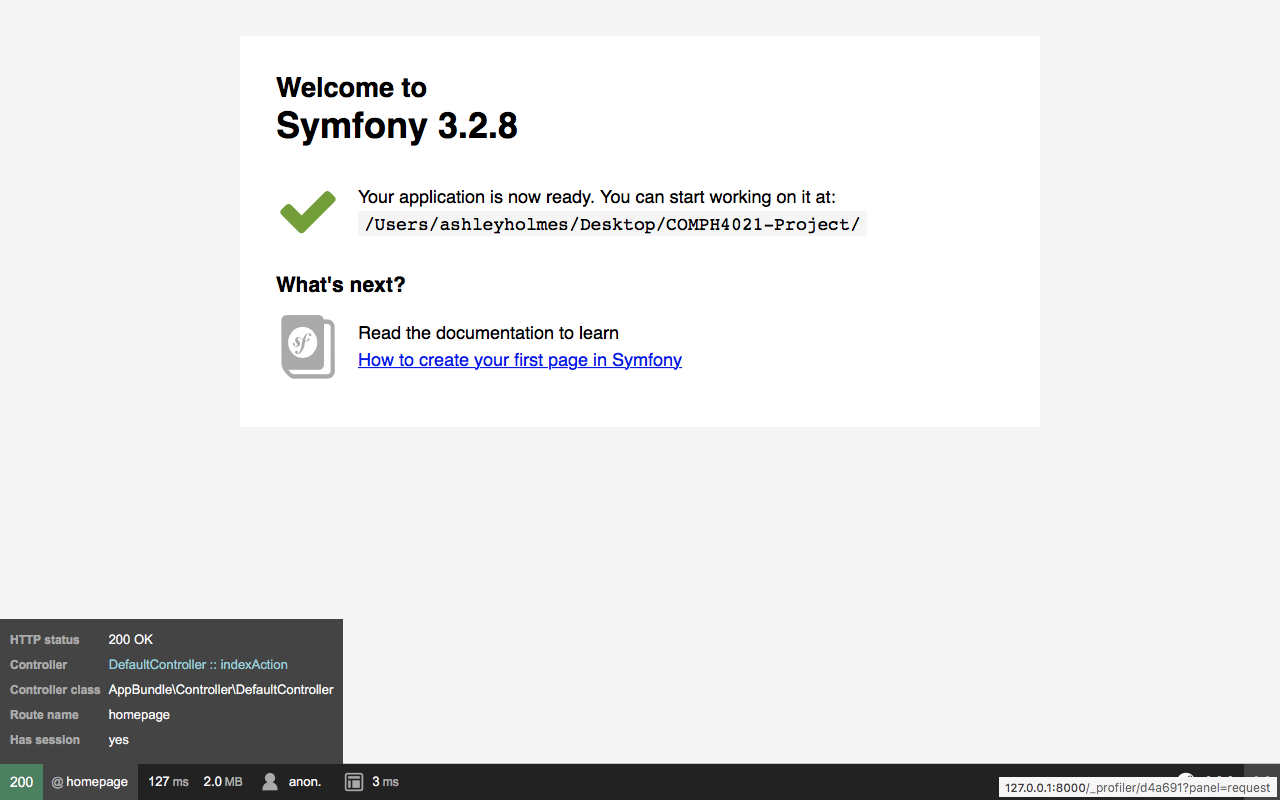
\includegraphics[width=400pt]{figures/webdebug_1.png}
   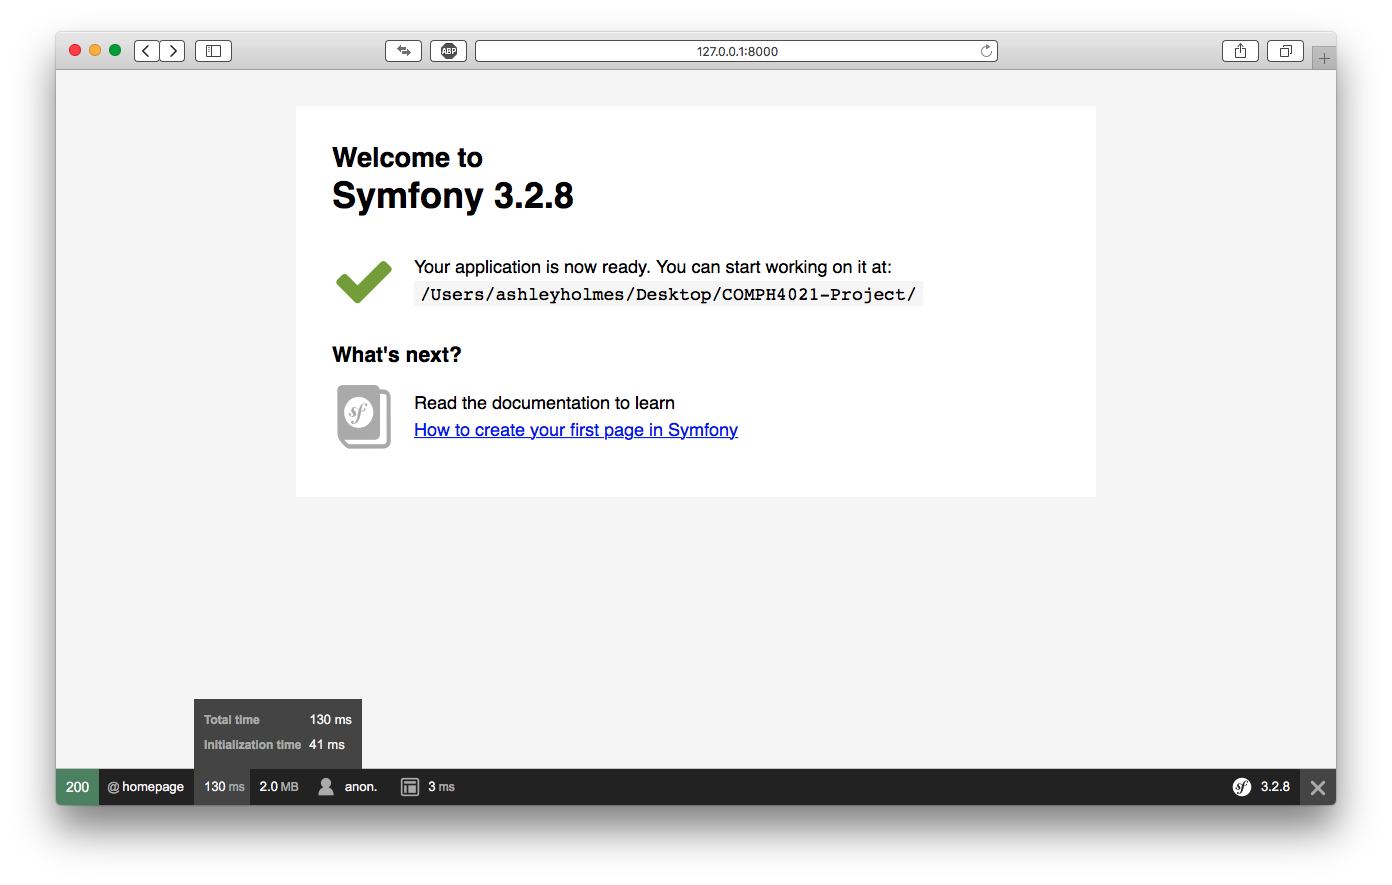
\includegraphics[width=400pt]{figures/webdebug_2.png} % requires the graphicx package
   \caption{Web Debug Toolbar and Profiler Extended}
   \label{fig:Web Debug Toolbar and Profiler Extended}
\end{figure}

\begin{figure}[htbp]
   \centering
   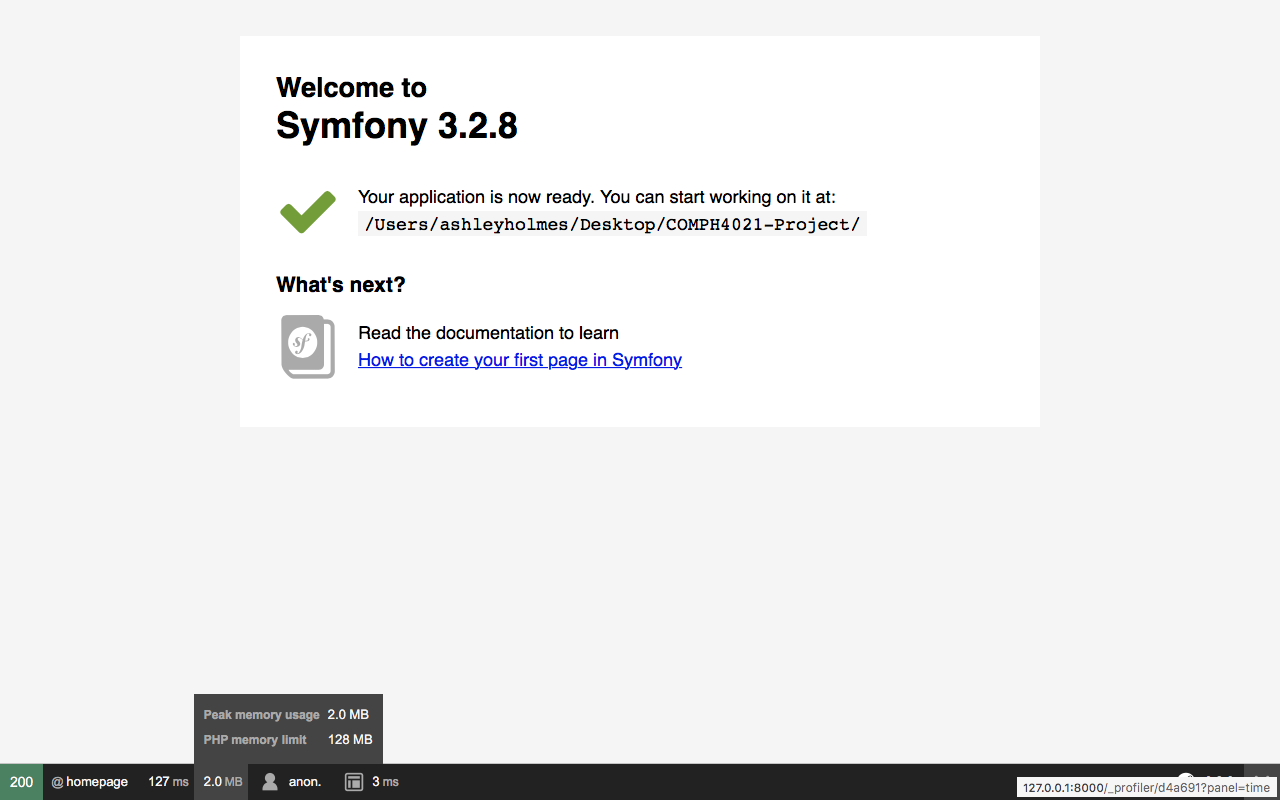
\includegraphics[width=400pt]{figures/webdebug_3.png} % requires the graphicx package
   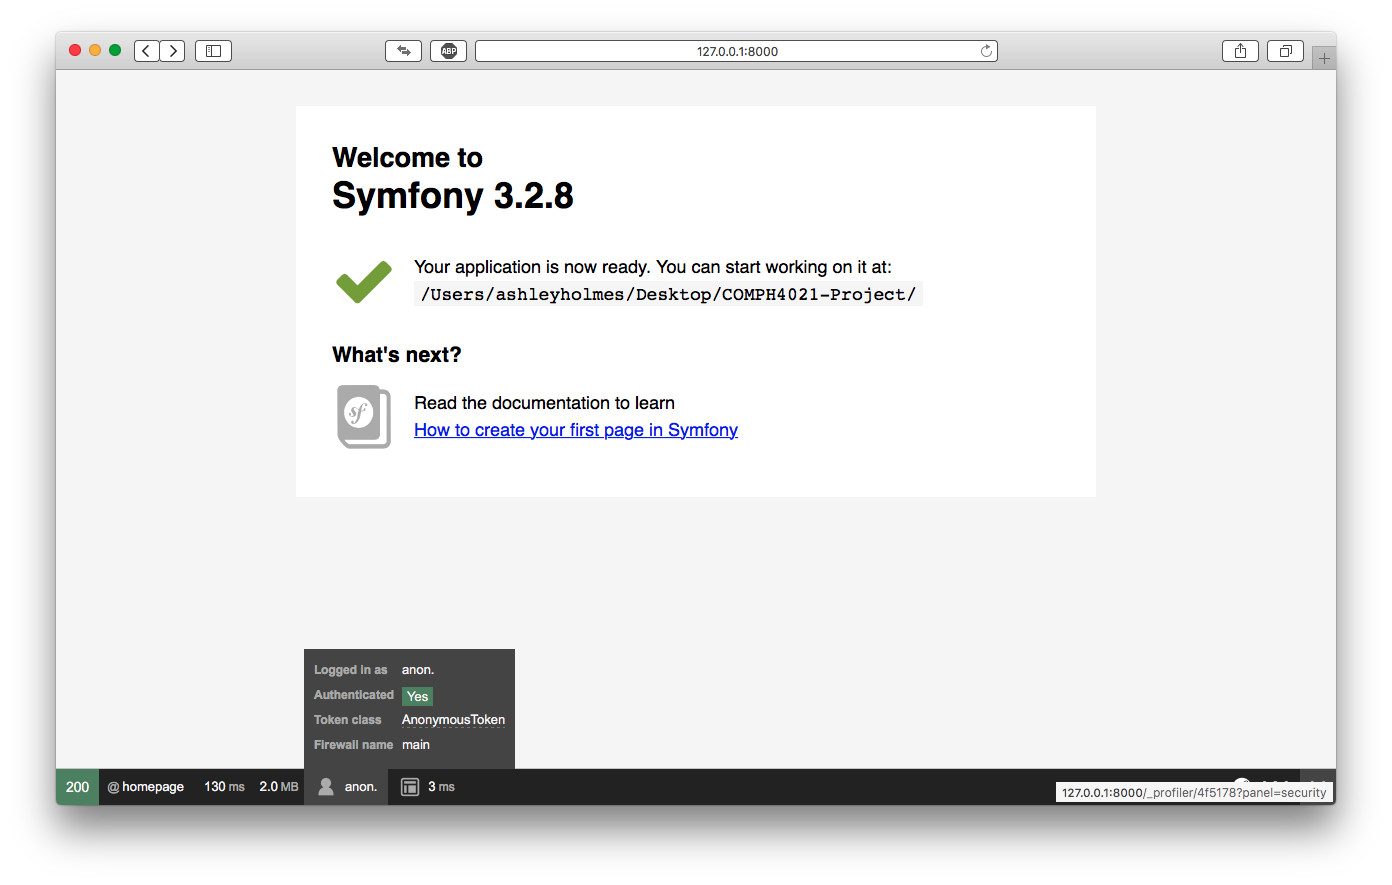
\includegraphics[width=400pt]{figures/webdebug_4.png}
   \caption{Web Debug Toolbar and Profiler Extended}
   \label{fig:Web Debug Toolbar and Profiler Extended}
\end{figure}

\begin{figure}[htbp]
   \centering
   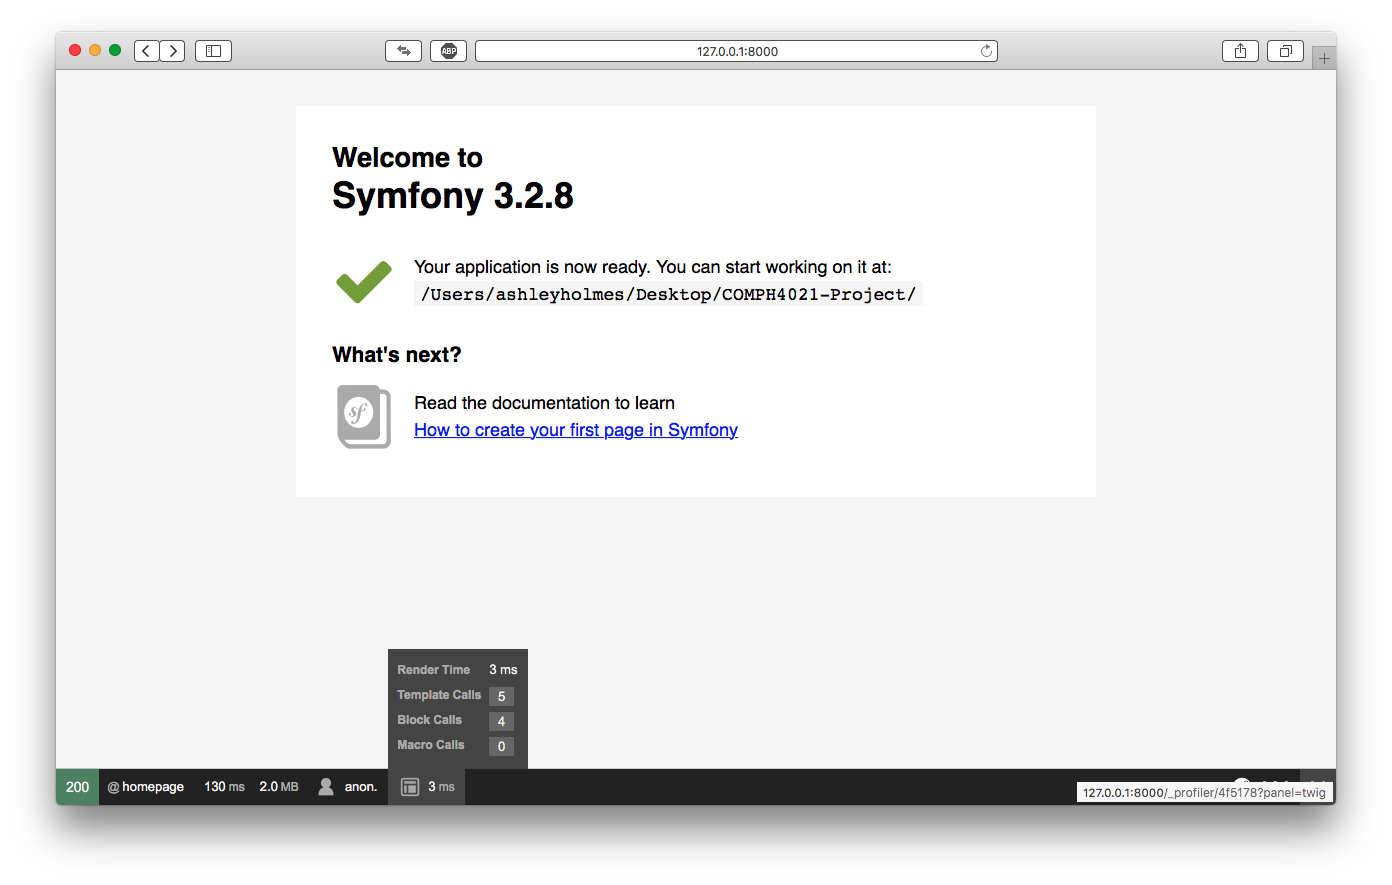
\includegraphics[width=400pt]{figures/webdebug_5.png}
   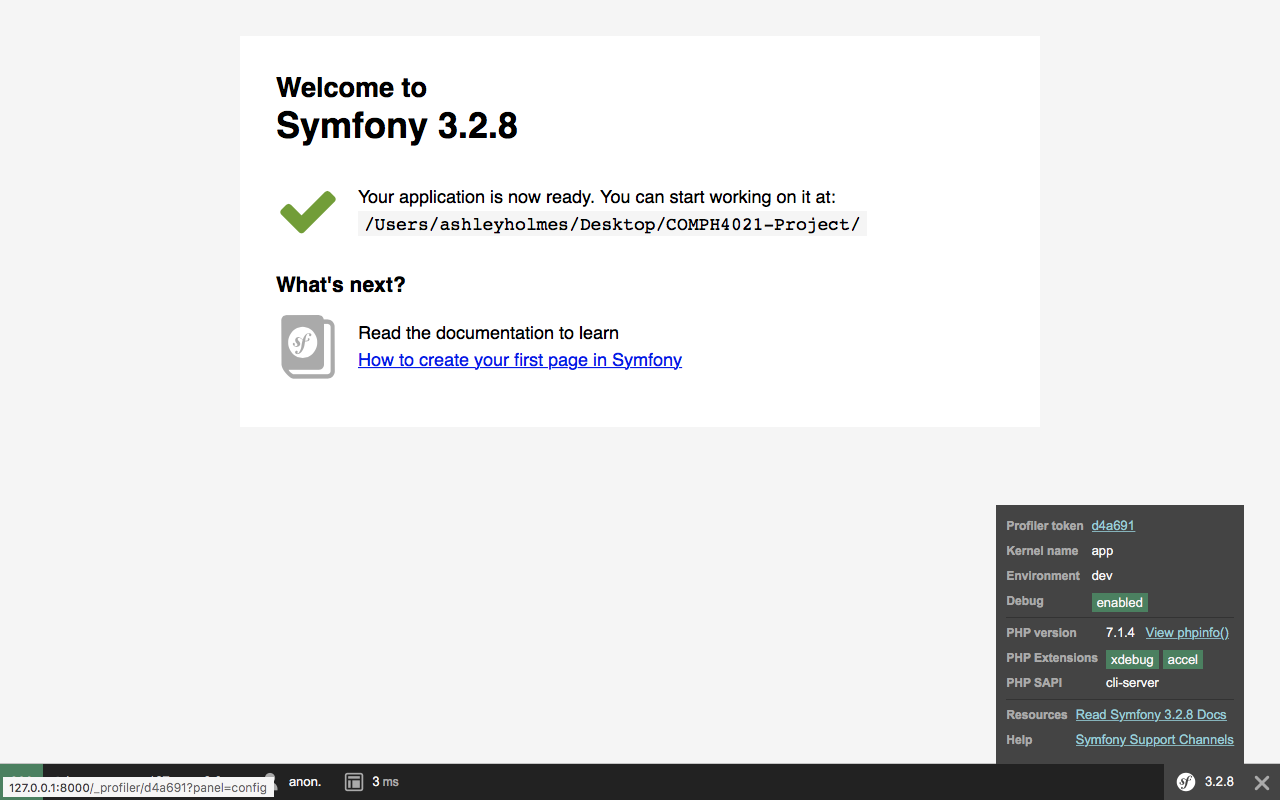
\includegraphics[width=400pt]{figures/webdebug_6.png} % requires the graphicx package
   \caption{Web Debug Toolbar and Profiler Extended}
   \label{fig:Web Debug Toolbar and Profiler Extended}
\end{figure}

Now that the configuration phase has been completed one now navigates to the browser and using the URL http://localhost:8000 as shown in the terminal window in figure \ref{fig:Terminal Window Bottom} under the Run your application heading. This brings up the following page in figure \ref{fig:Symfony Browser}. It is being executed by the Symfony framework from the files inside the project folder. The code is depicted in figure \ref{fig:Web Debug Toolbar and Profiler}. In the bottom of the window is the web debug toolbar which is in a maximised position and can be minimised by clicking on the X in the right hand corner. This often offers better visibility when developing. If the mouse is used to hover over the toolbar it will display information such as routing, controllers which were executed, time it took to load the page, which way the user is authenticated on the page and more debugging information and a link to the resources and documentation as shown in figure \ref{fig:Web Debug Toolbar and Profiler Extended}. Clicking on the icons will give much more information. The URL http://127.0.0.1:8000/config.php would show the user the instructions needed for further configuration. This is reference to figure \ref{fig:Configuration Checker}.


\begin{figure}[htbp]
   \centering
   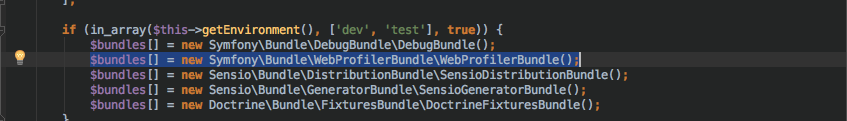
\includegraphics[width=400pt]{figures/AppKernel.png}
   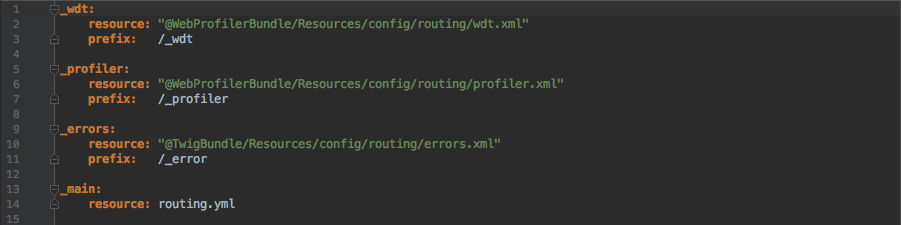
\includegraphics[width=400pt]{figures/routing_dev.png}
   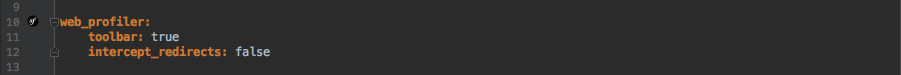
\includegraphics[width=400pt]{figures/config_dev.png} % requires the graphicx package
   \caption{Web Debug Toolbar and Profiler}
   \label{fig:Web Debug Toolbar and Profiler}
\end{figure}

\section{IDE}

\subsection{PhpStorm IDE for PHP}

Most of the files live in src/AppBundle. Looking at the controller called DefaultController in the below figure \ref{fig:DefaultController}. This controller class defines what is seen in figure \ref{fig:Symfony Browser}. It renders the Symfony Welcome Page. Take note of the @Route("/", name="homepage") annotation on line 12. It matches the route in figure \ref{fig:Web Debug Toolbar and Profiler Extended}. The next process was to remove the extraneous code which was not needed in the Twig template and the DefaultController. In the template itself, it was using some variables which was passed in line 18 of figure \ref{fig:DefaultController} in the\newline DefaultController.php class. With this removed, Bootstrap was enabled as a CDN and added to the templates to provide consistency across all pages. In order to use Bootstrap, it needed to be downloaded from the Bootstrap website. From the Getting started section there are examples which can be chosen as a starting template to use as a foundation for all templates. This was added to the base.html.twig and then modified to make it more specific to the project. Twig uses inheritance and all templates extend from the base.html.twig. In addition to this a small amount of custom CSS was added to achieve the result in figure \ref{fig:Home Page}

\begin{figure}[htbp]
   \centering
   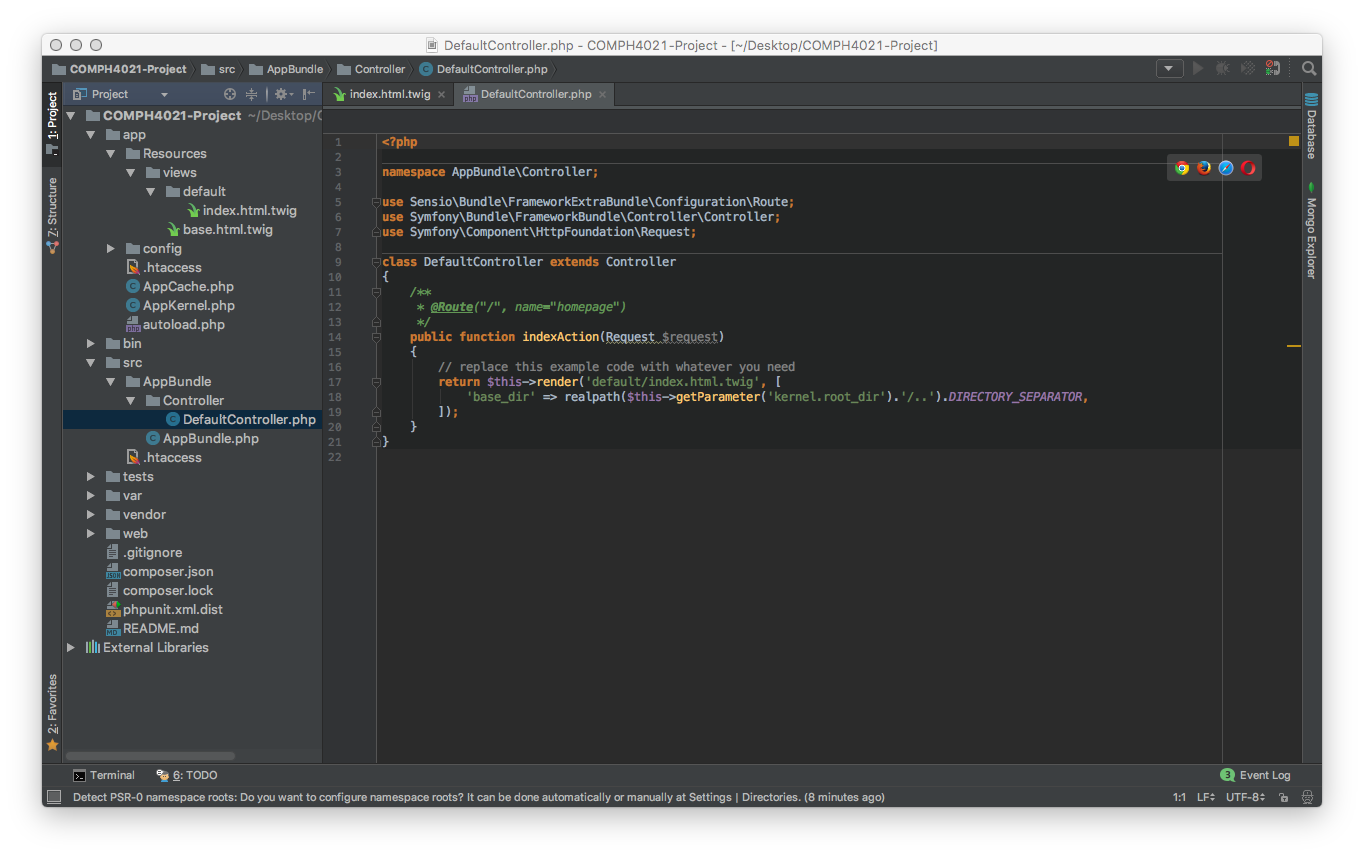
\includegraphics[width=400pt]{figures/default_controller.png} % requires the graphicx package
   \caption{DefaultController}
   \label{fig:DefaultController}
\end{figure}

\begin{figure}[htbp]
   \centering
   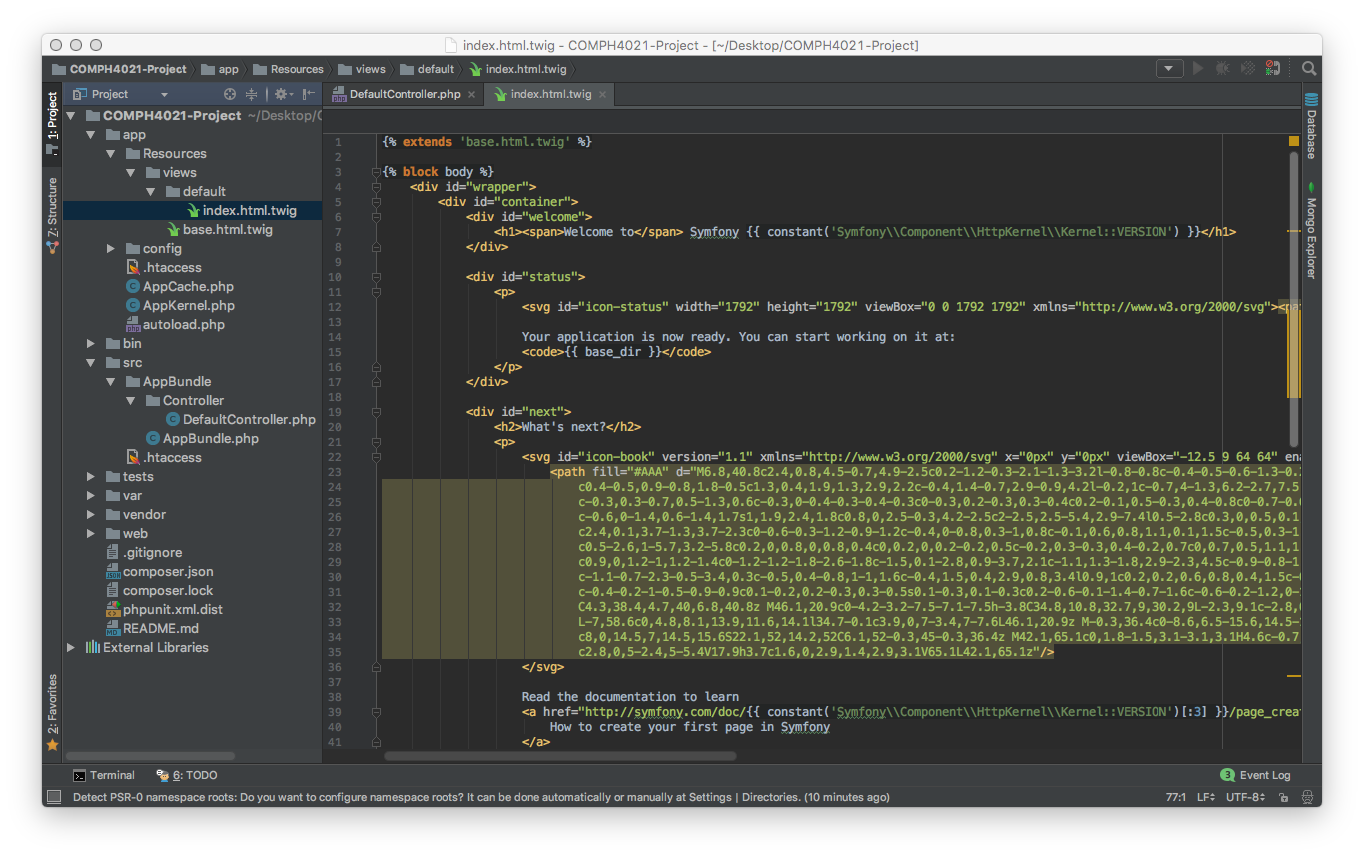
\includegraphics[width=400pt]{figures/twig_index.png} % requires the graphicx package
   \caption{Twig template in IDE}
   \label{fig:Twig template in IDE}
\end{figure}

\begin{figure}[htbp]
   \centering
   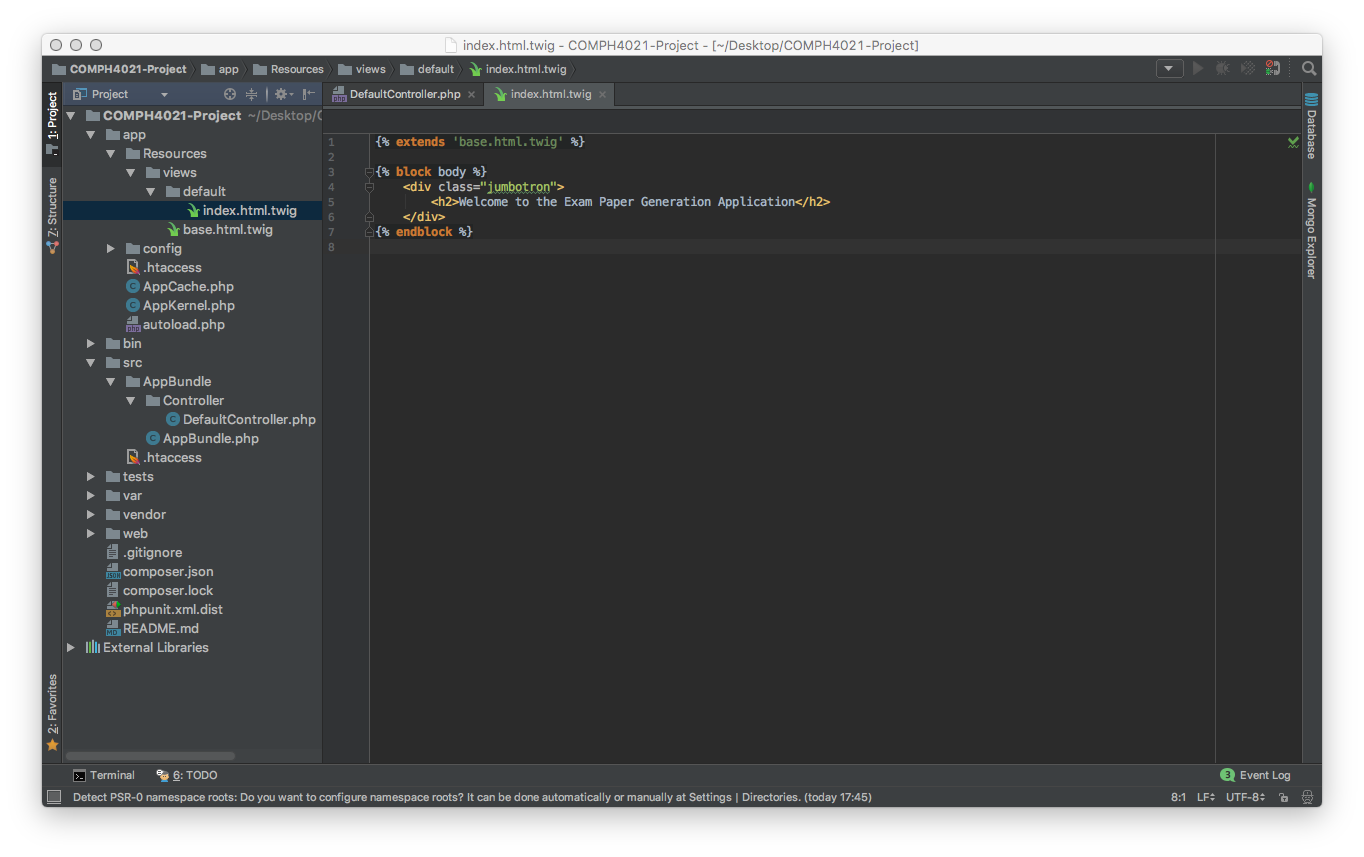
\includegraphics[width=400pt]{figures/index_html.png} % requires the graphicx package
   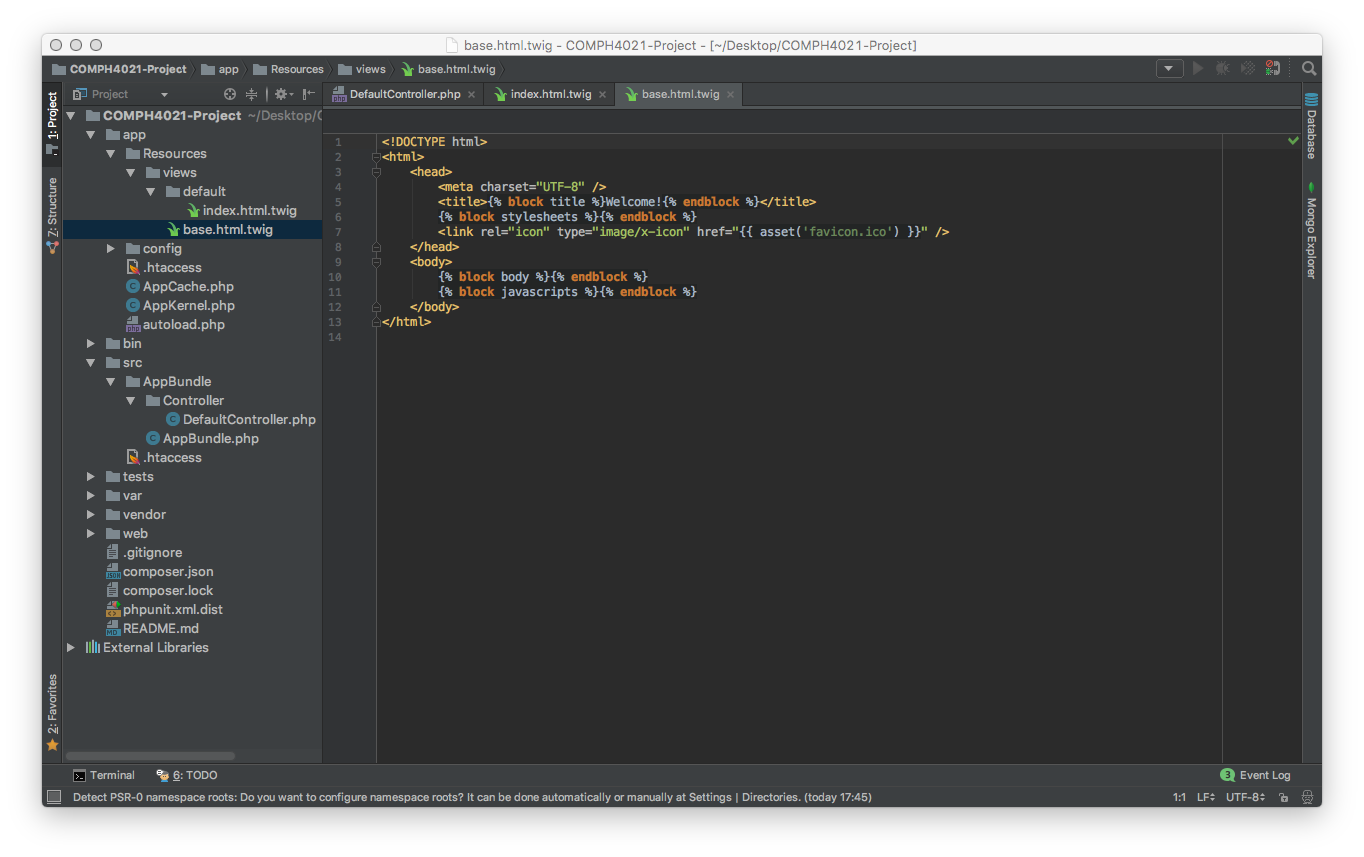
\includegraphics[width=400pt]{figures/base_html.png}
   \caption{Adding Bootstrap}
   \label{fig:Adding Bootstrap}
\end{figure}

\begin{figure}[htbp]
   \centering
   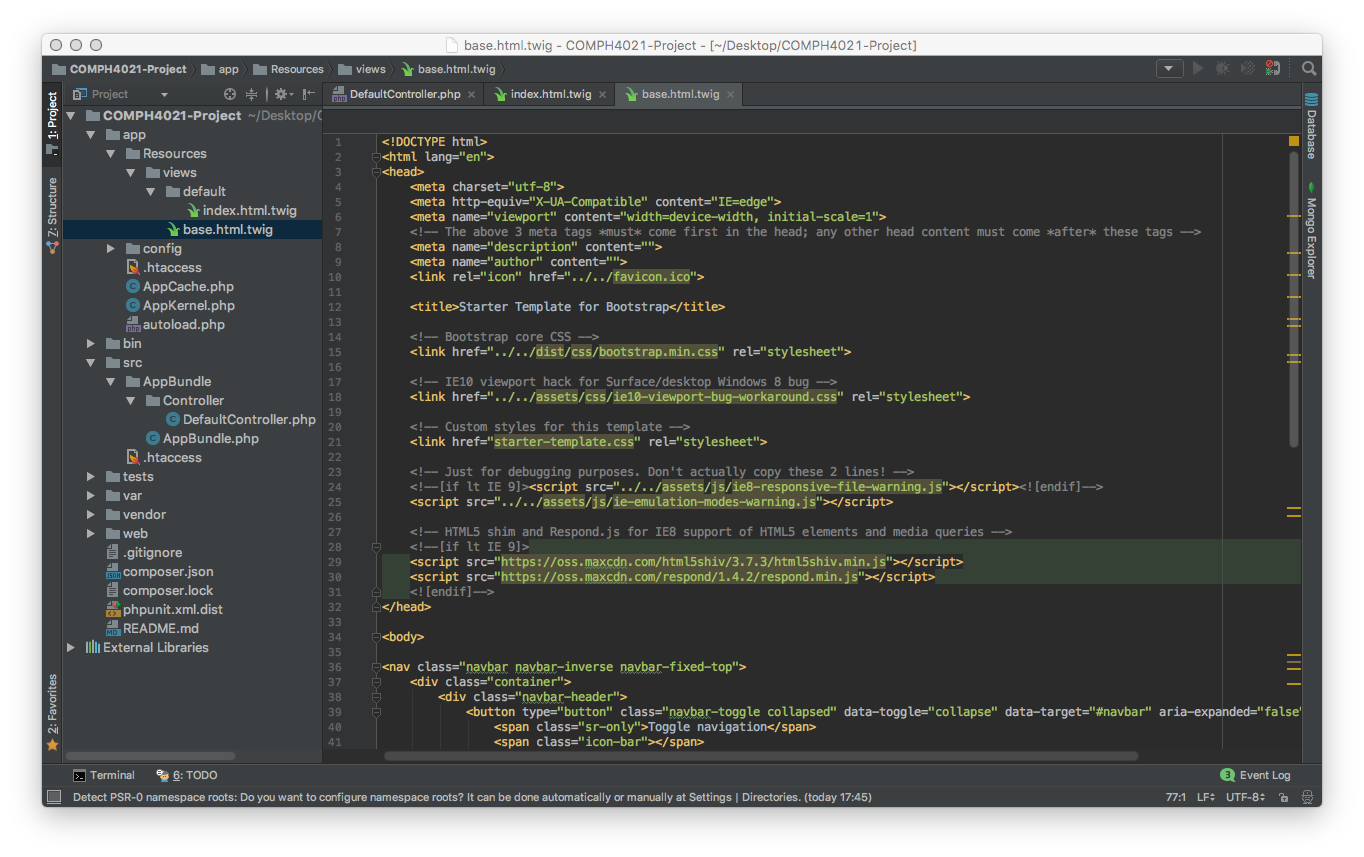
\includegraphics[width=400pt]{figures/bootstrap_html.png} % requires the graphicx package
   \caption{Adding Bootstrap}
   \label{fig:Adding Bootstrap}
\end{figure}

\begin{figure}[htbp]
   \centering
   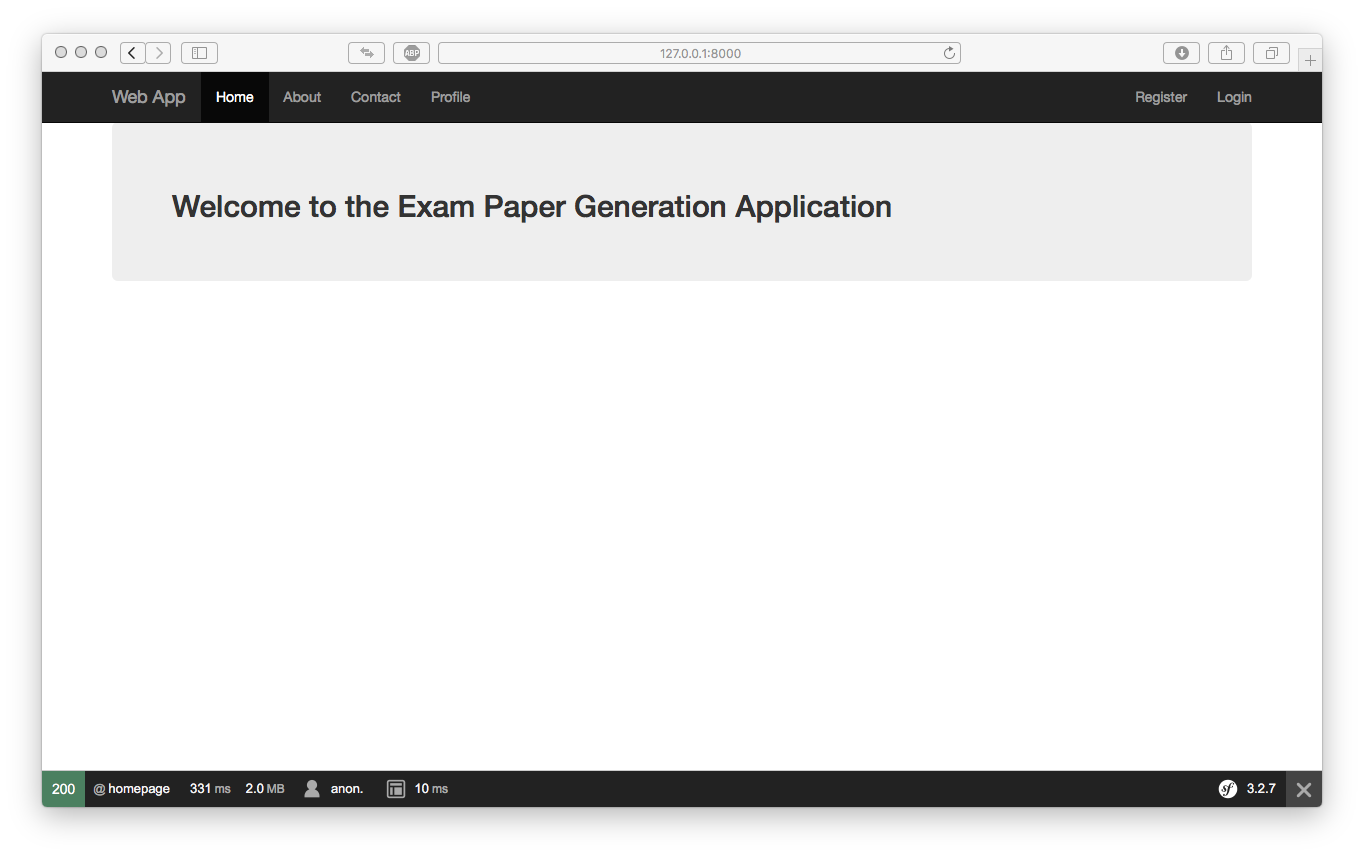
\includegraphics[width=400pt]{figures/homepage.png} % requires the graphicx package
   \caption{Home Page}
   \label{fig:Home Page}
\end{figure}

\section{Database}

\subsection{Creation of User Entity and CRUD}

\begin{figure}[htbp]
   \centering
   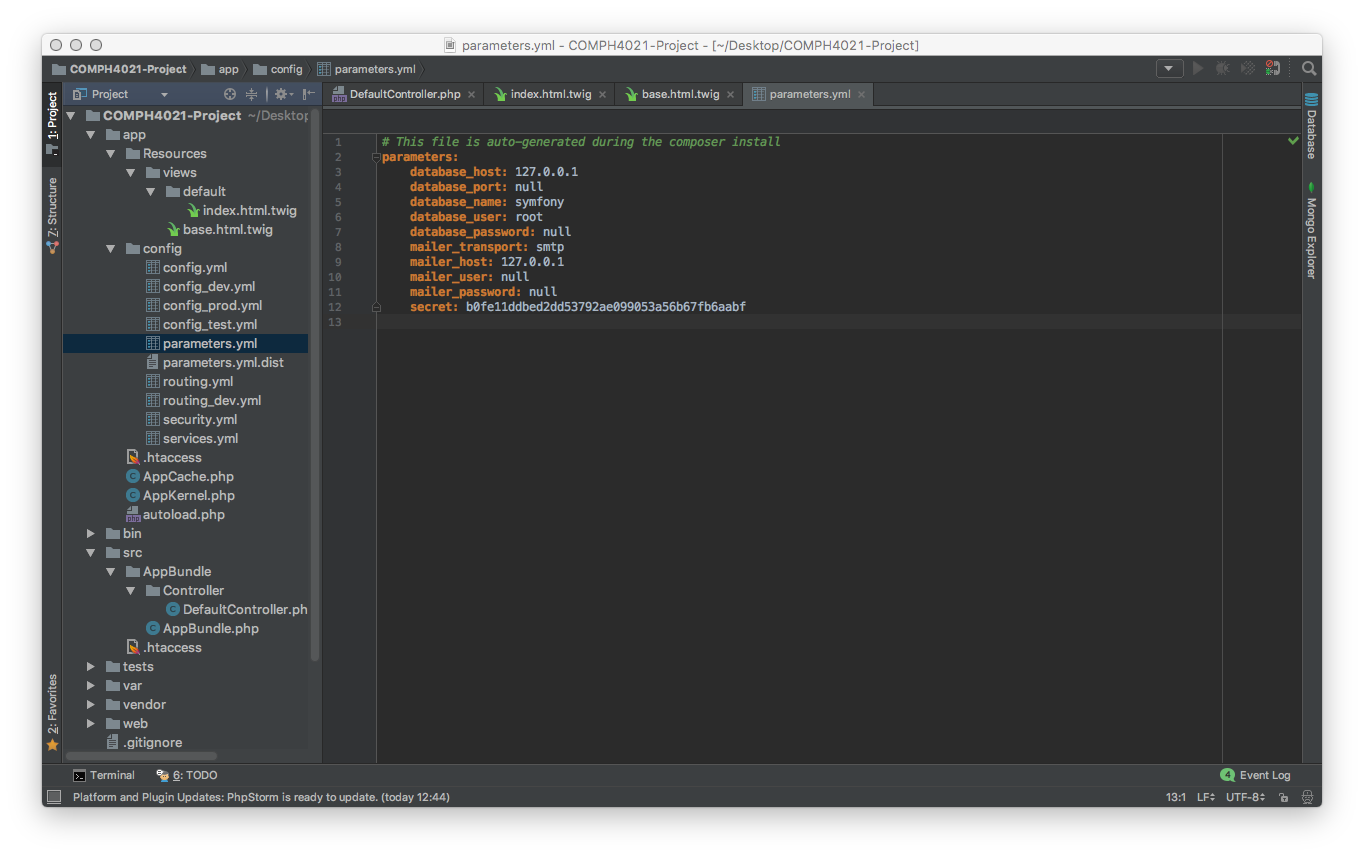
\includegraphics[width=400pt]{figures/entity_crud.png} % requires the graphicx package
   \caption{Parameters Yaml}
   \label{fig:Parameters Yaml}
\end{figure}

This section covers Object Relational Mapping or ORM. With using an ORM, the concept of working with a database becomes easier as it is an easy switch from one to another such as Mongo to SQL or Postgres. Not having to worry about the actual database. Symfony takes care of the abstraction. In addition the ORM generates the CRUD off the entity which is made and makes everything work. The first thing that needs to be done is make a change to the parameters.yml which can be seen in figure \ref{fig:Parameters Yaml}. The change was to the database name from symfony in line 5 to a name of choice. In this case the name project was used. The database port changed to 8889 and the database password changed to root to correspond with the database login details. With having done that an external MySQL server was needed to make a communication to the database itself. The port number is the port on the local MySQL server. In this case MAMP was used in figure \ref{fig:Mamp Ports}. 

\begin{figure}[htbp]
   \centering
   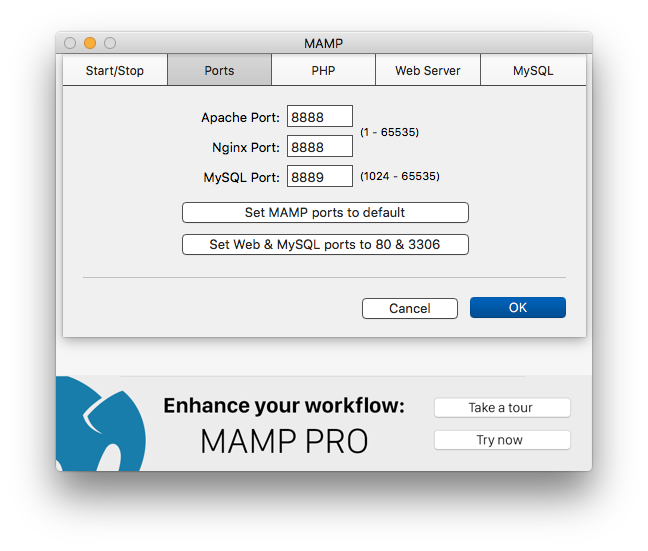
\includegraphics[width=400pt]{figures/mamp_ports.png} % requires the graphicx package
   \caption{Mamp Ports}
   \label{fig:Mamp Ports}
\end{figure}

\begin{figure}[htbp]
   \centering
   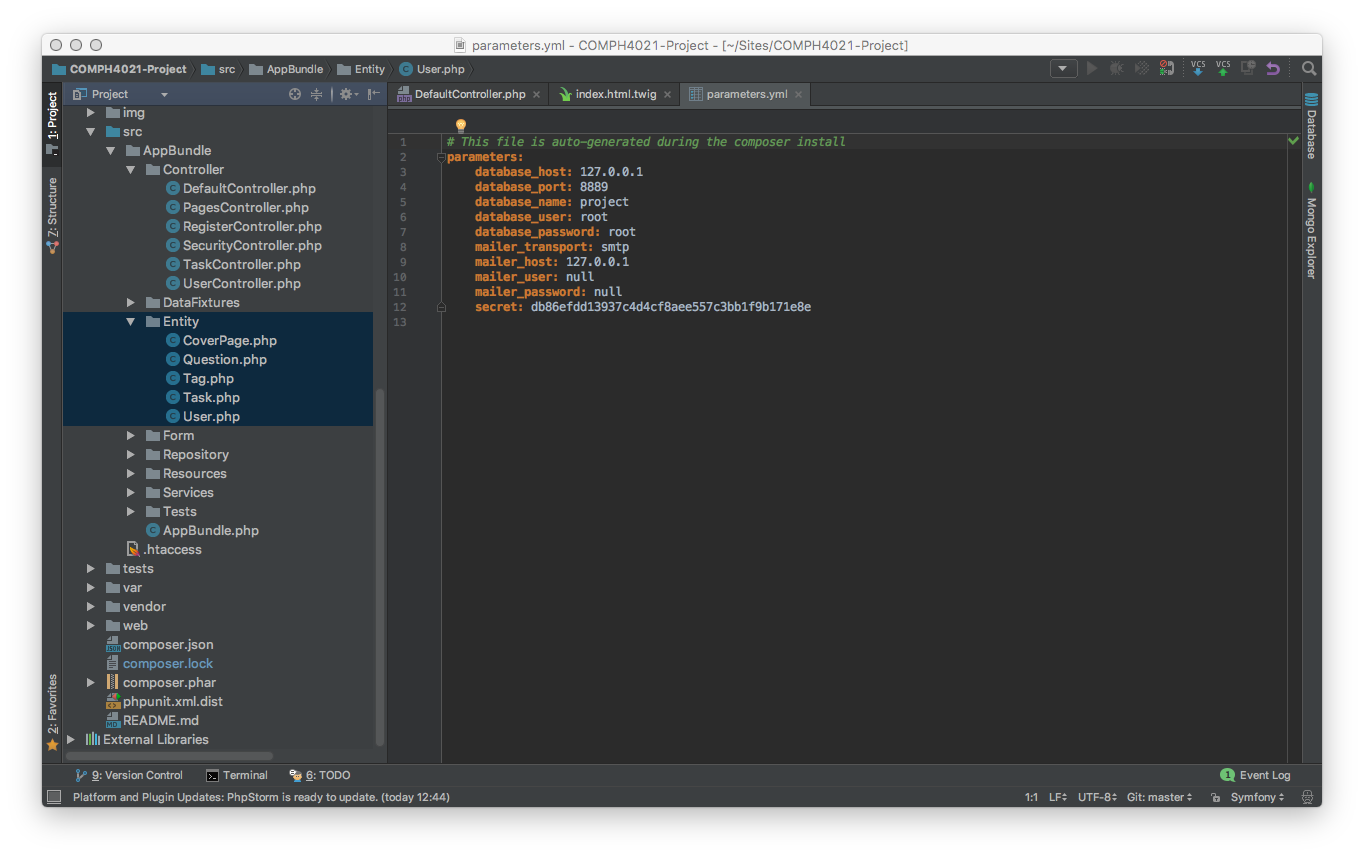
\includegraphics[width=400pt]{figures/entities.png} % requires the graphicx package
   \caption{Entities}
   \label{fig:Entities}
\end{figure}

\begin{figure}[htbp]
   \centering
   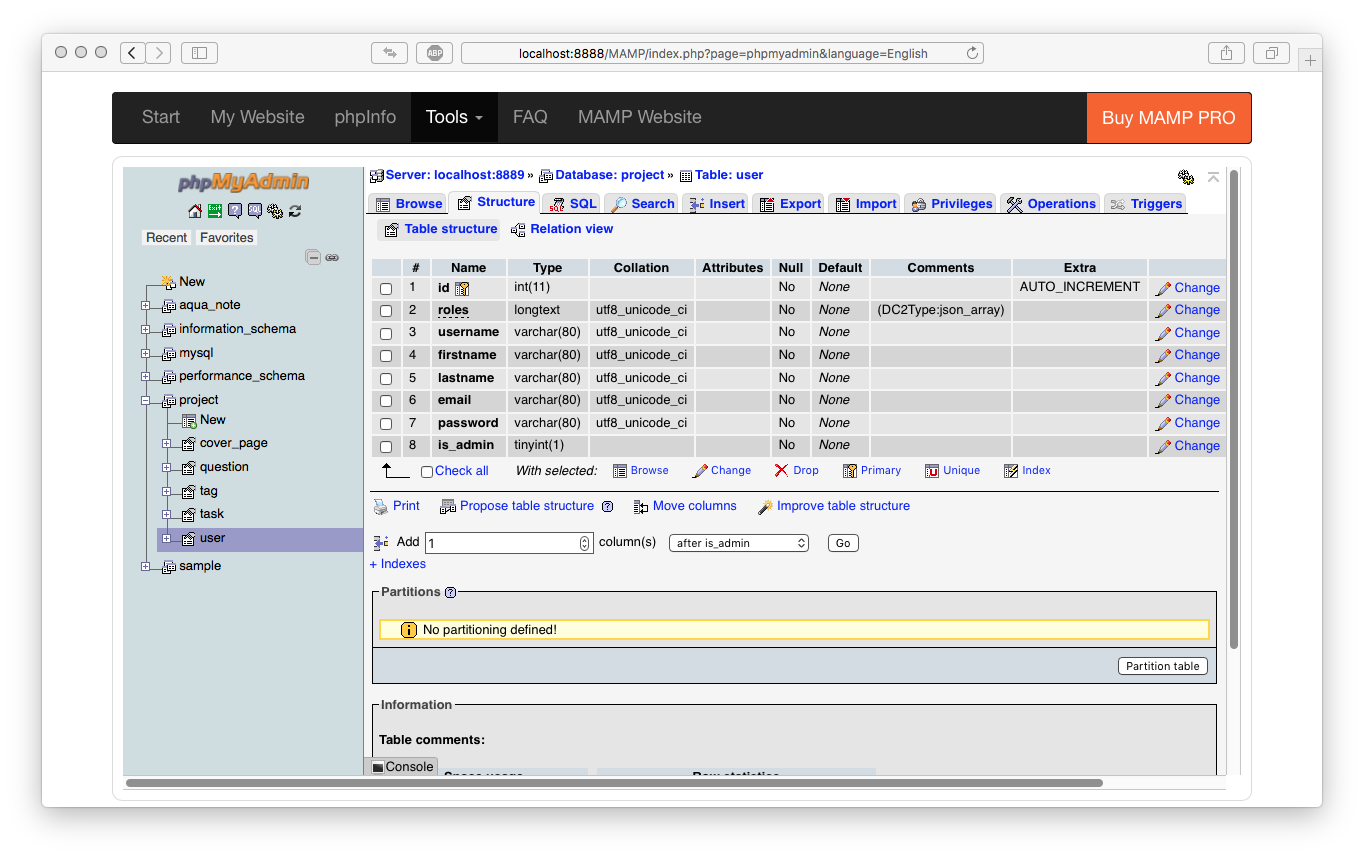
\includegraphics[width=400pt]{figures/tables_user_entity.png} % requires the graphicx package
   \caption{User Table}
   \label{fig:User Table}
\end{figure}

\begin{figure}[htbp]
   \centering
   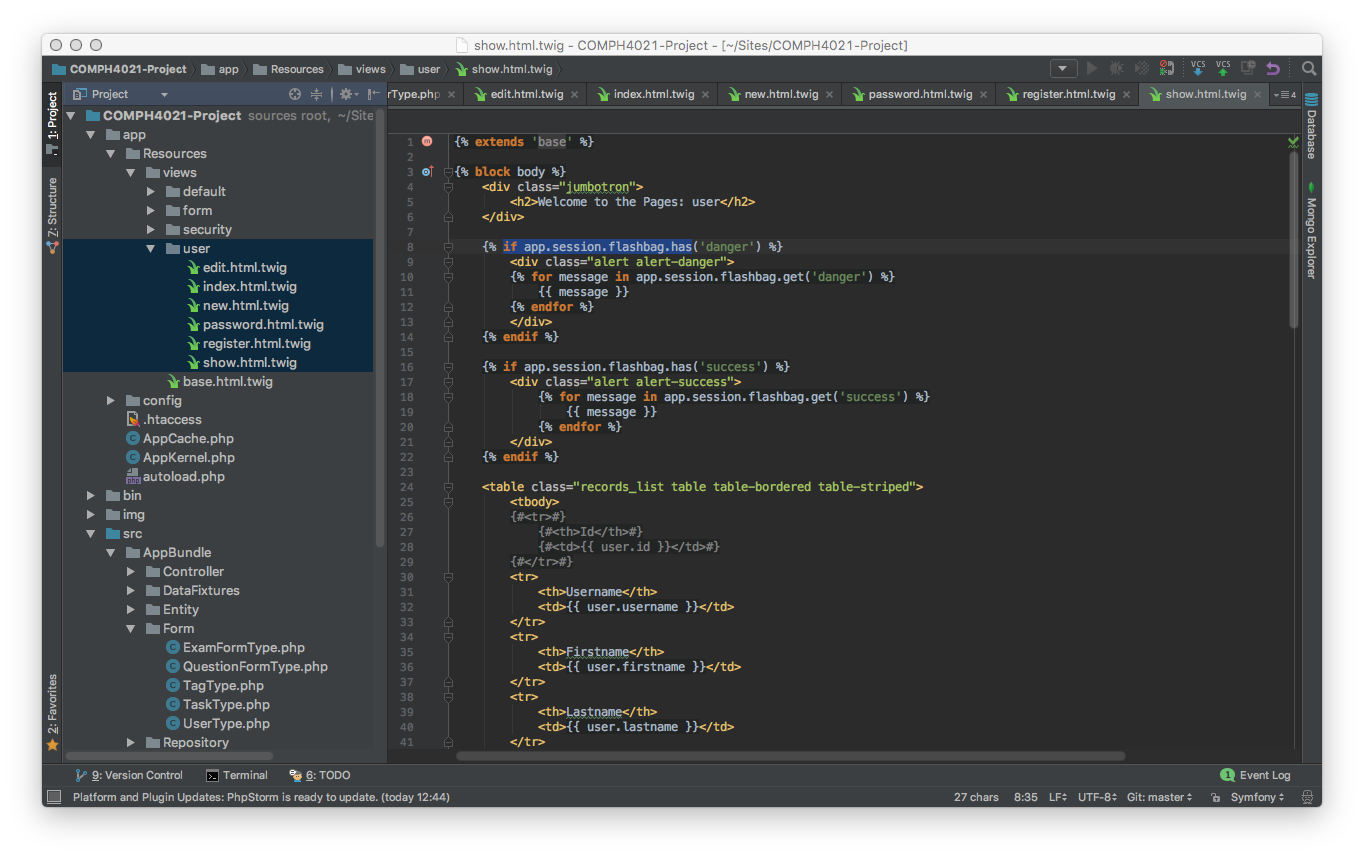
\includegraphics[width=400pt]{figures/templates.png} % requires the graphicx package
   \caption{Twig templates}
   \label{fig:Twig templates}
\end{figure}

\begin{figure}[htbp]
   \centering
   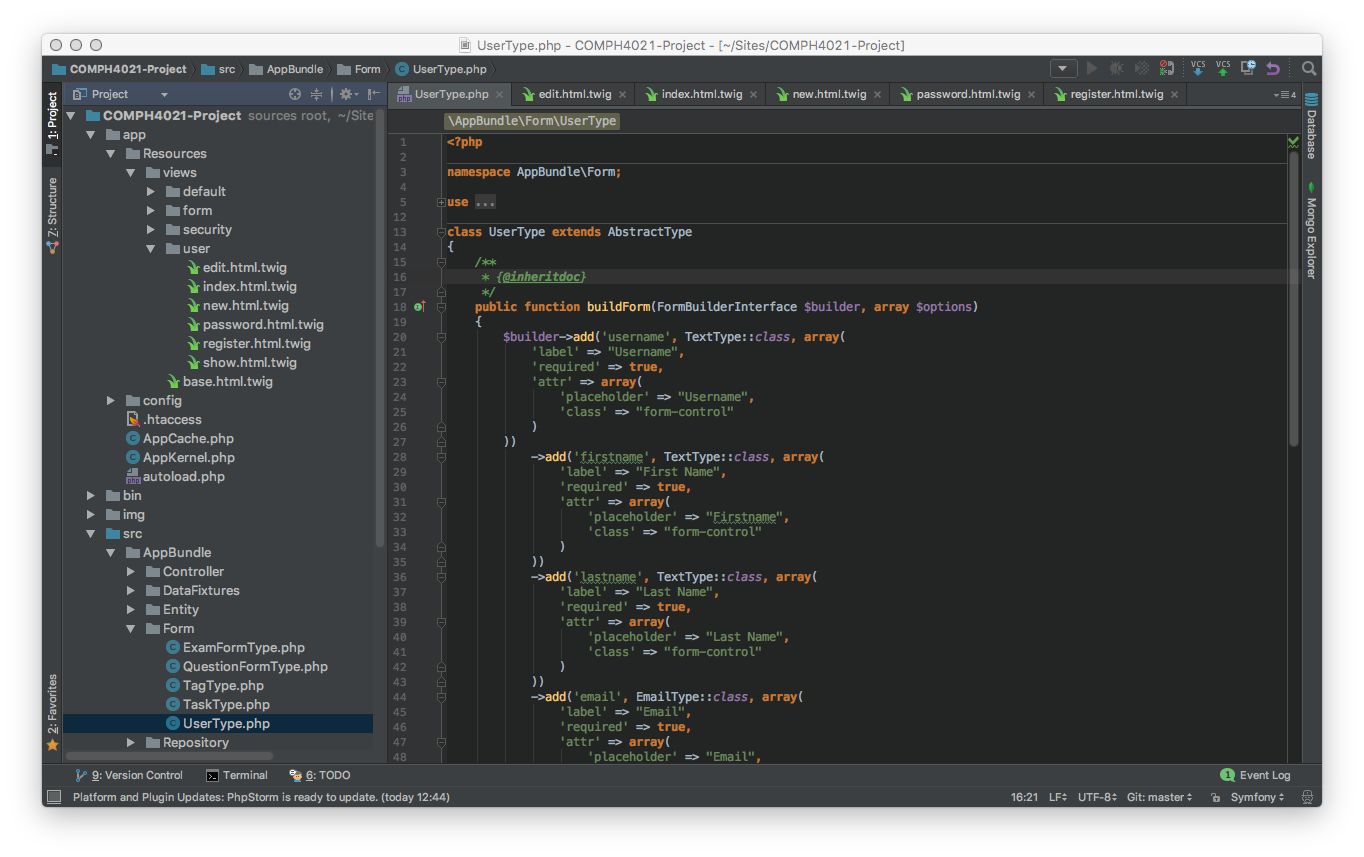
\includegraphics[width=400pt]{figures/form_type.png} % requires the graphicx package
   \caption{Form Type}
   \label{fig:Form Type}
\end{figure}

Issuing a command in the terminal. php bin/console doctrine:database:create will create a database with the name project which was added to the parameters.yml file. Creating the entities is done in the same manor. php bin/console doctrine:generate:entity brings up a wizard which asks where to put the entity. Giving the command AppBundle:User. The entities were all placed in a directory called Entity which resides in src/AppBundle. All the work was was done is in AppBundle. The fields in the database are then added along with a repository class which will be discussed later. There is now a username, firstname, lastname, email and password with type String and field length of 80 characters. An example of this is in figure \ref{fig:User Table}. Symfony created two different files. The first is the user entity which is the model which is used to base database manipulation, object validation or form validation. The second thing which was done was to create the schema which is done in the terminal with the command of php bin/console doctrine:schema:create. This creates a table structure ready for use off of the user object. To create the CRUD in the terminal it was php bin/console generate:doctrine:crud. The wizard asks where the entity would be found and based off. As discussed it is in AppBundle:User and giving write actions which allows for the update and delete. All the templates were created and added to the Resources directory which are used to create the users in figure \ref{fig:Twig templates} also a class called UserType.php which is a FormType and is what all the forms are based off in figure \ref{fig:Form Type}. With this section completed a bit of functional testing was done to make sure that users could be added to the database, edited and removed.

\section{Twig}

\subsection{Templates are fine tuned}

The templates which are created by Symfony was raw html with no styling. Each form had a basic layout. They were ugly. This is why form theming which is discussed later in the chapter and styling needed to be added to make them look as they do in the below figures. Styling included:

\begin{itemize}
  \item Addition of placeholders.
    \item Adding a striped table.
      \item Button styling.
        \item Removal of the unordered lists.
          \item Adding column spanning.
            \item Changing links to be buttons.
              \item The bootstrap classes were added.
                \item Button styling.     
\end{itemize}

Some of the data was adjusted which would have been displayed such as the id and passwords which were removed as they should not be visible from the client side.

\begin{figure}[htbp]
   \centering
   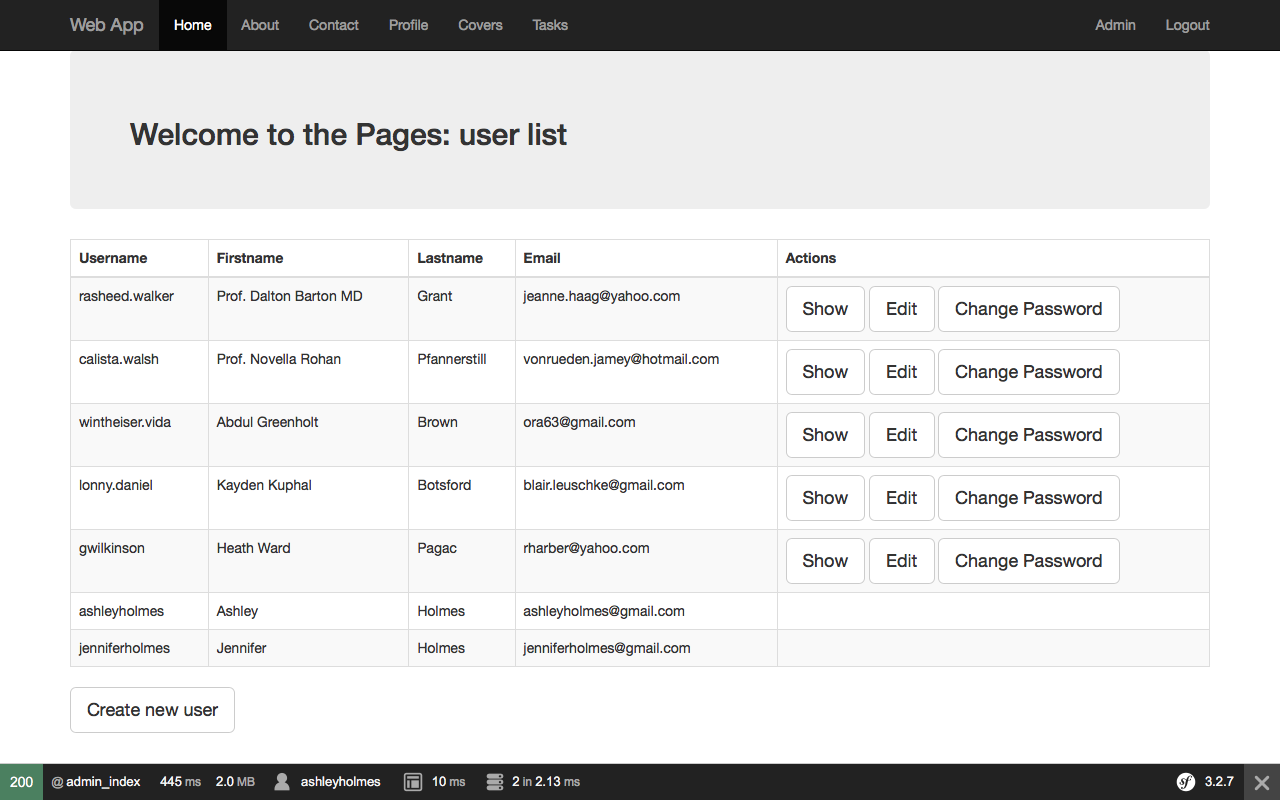
\includegraphics[width=400pt]{figures/index_html_twig.png} % requires the graphicx package
   \caption{index.html.twig}
   \label{fig:index.html.twig}
\end{figure}

\begin{figure}[htbp]
   \centering
   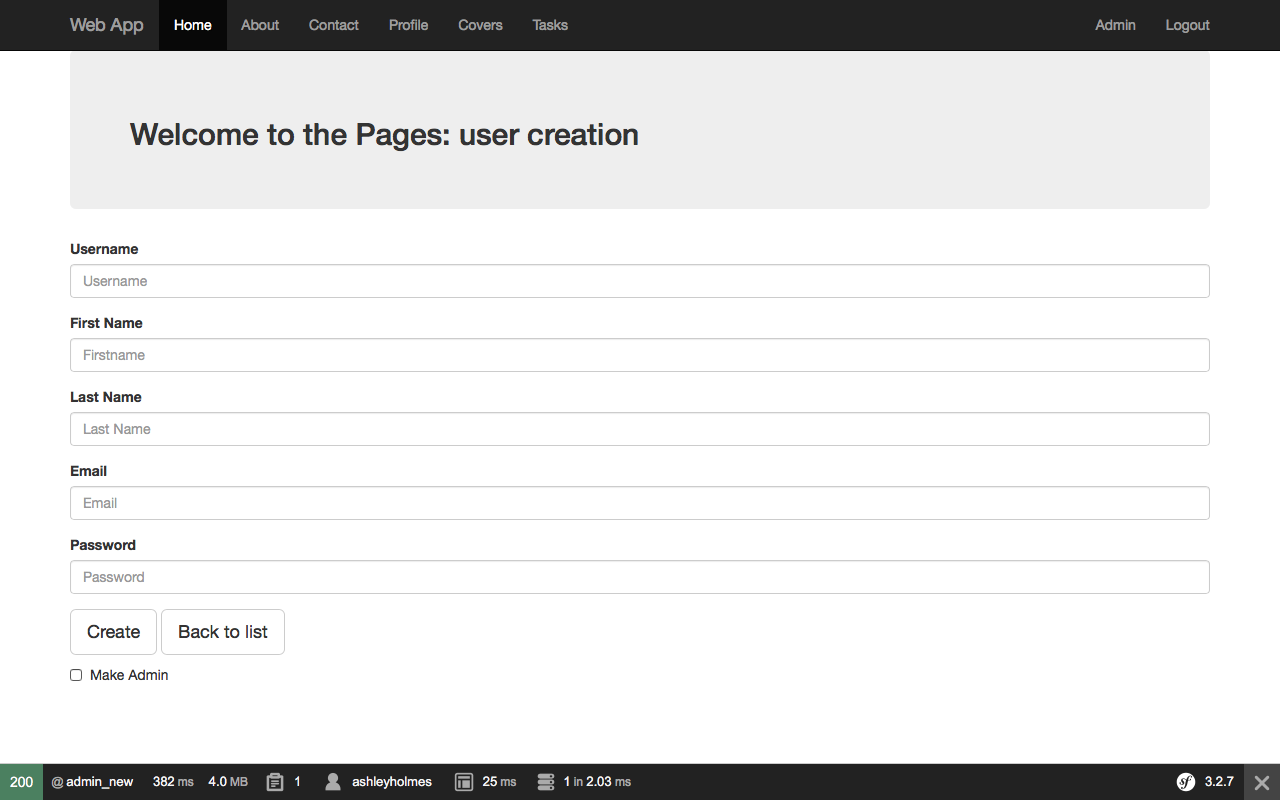
\includegraphics[width=400pt]{figures/new_html_twig.png} % requires the graphicx package
   \caption{new.html.twig}
   \label{fig:new.html.twig}
\end{figure}

\begin{figure}[htbp]
   \centering
   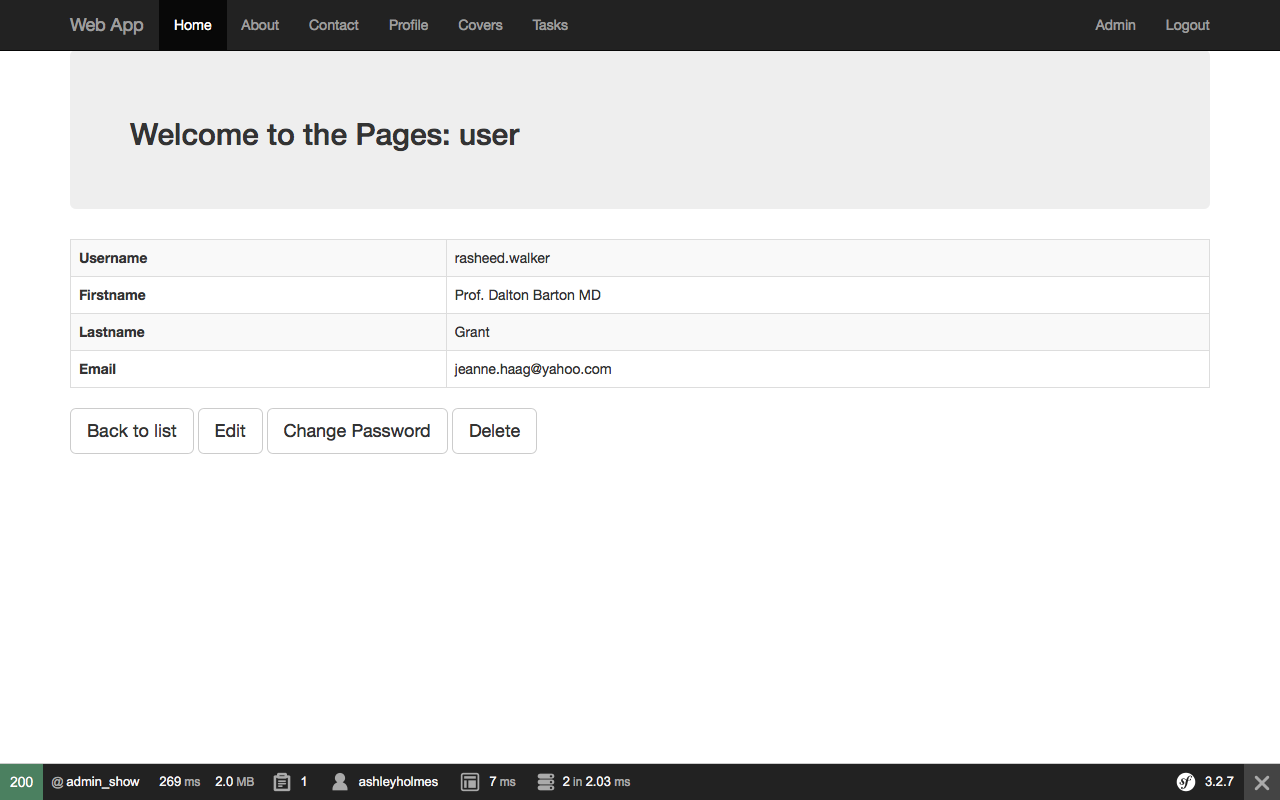
\includegraphics[width=400pt]{figures/show_html_twig.png} % requires the graphicx package
   \caption{show.html.twig}
   \label{fig:show.html.twig}
\end{figure}

\begin{figure}[htbp]
   \centering
   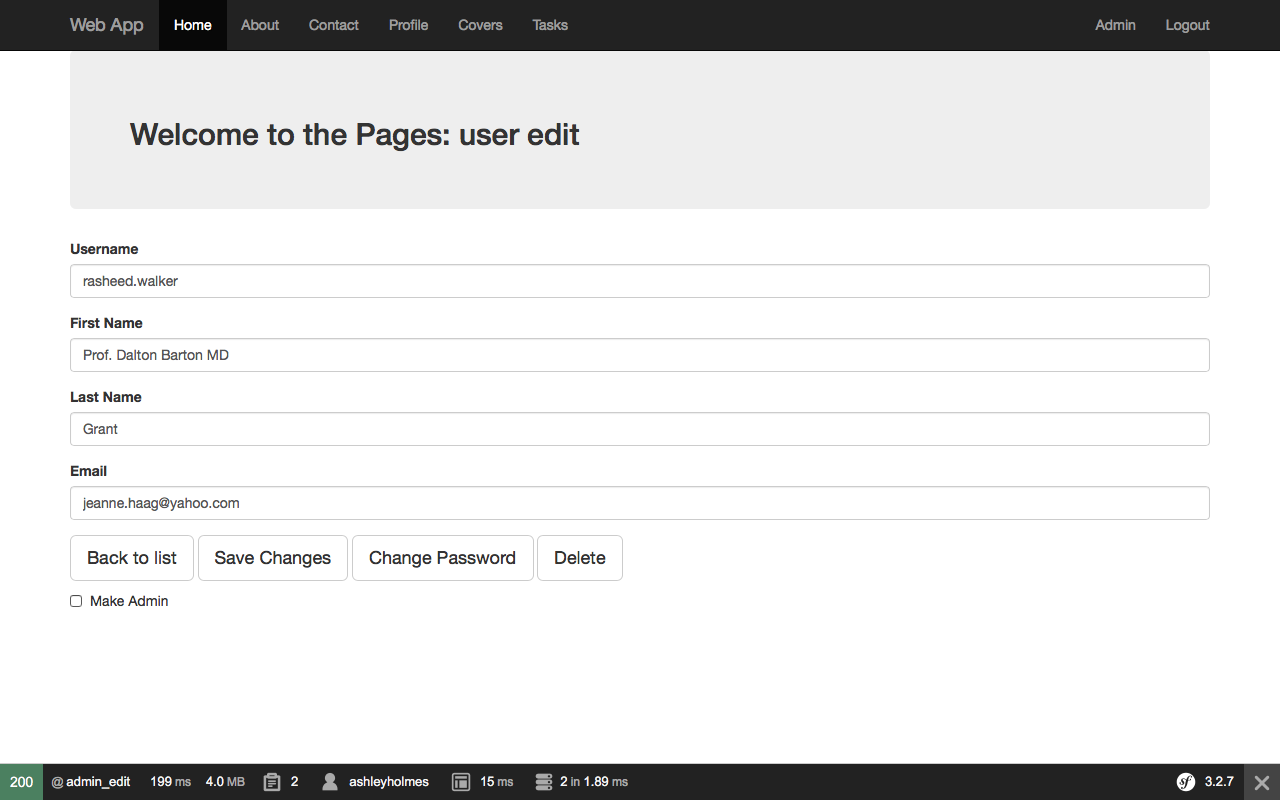
\includegraphics[width=400pt]{figures/edit_html_twig.png} % requires the graphicx package
   \caption{edit.html.twig}
   \label{fig:edit.html.twig}
\end{figure}

\section{Forms}

\subsection{Understanding FormTypes}

The FormType works hand in hand with the user object which is created and thus is called the UserType which can be found in src/AppBundle/Form/UserType.php. This is what Symfony created when going through the process of creating CRUD. The FormType is used to take control of the input tags and labels. As mentioned in the previous Twig section with regards to adding the placeholders. This is actually done in the UserType.php class including the CSS classes. When the user clicks on the Create new user button. Symfony extracts information from that FormType and it builds the form. In figure \ref{fig:UserType.php} one can see that the add method takes up to three arguments. If only one argument is added, Symfony will make the best guess about what is being done. If the second argument is passed in, the second argument is the type of input that is being provide. It could take an Entity or several other arguments. However it does help Symfony make a better decision about what is being done. The third argument is where one can explicitly say what the options are such as input tags a class as mentioned before. When an array of options are provided Symfony stops guessing what is being done and it takes explicit direction. This is why an array of options are given to explicitly say everything. From line 20 to 25 there is an array of options such as:

\begin{figure}[htbp]
   \centering
   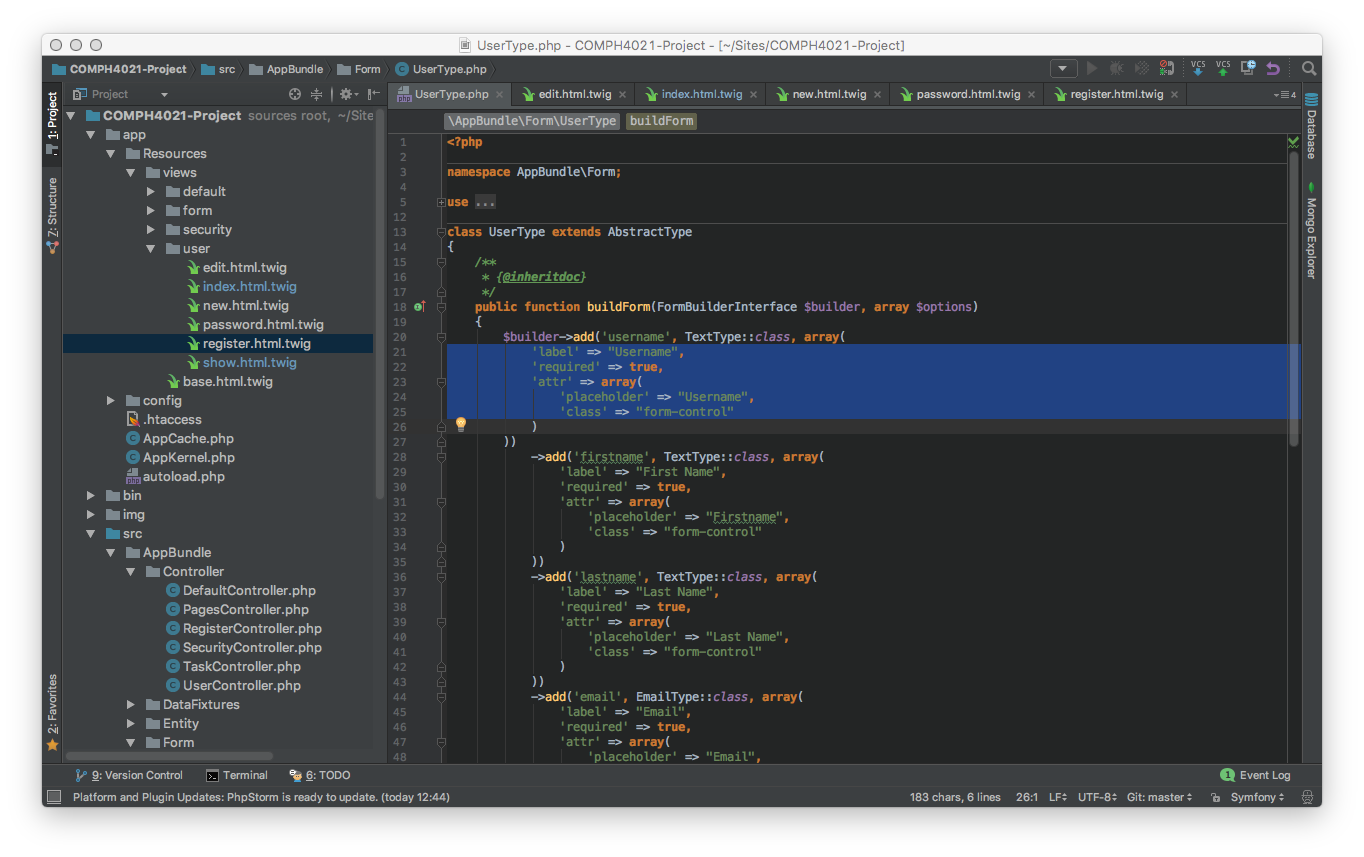
\includegraphics[width=400pt]{figures/userType.png} % requires the graphicx package
   \caption{UserType.php}
   \label{fig:UserType.php}
\end{figure}

\begin{itemize}
  \item The input label - is expressly put in with the form rendering where in the Twig template figure \ref{fig:Form Label} line 12, 17, 22, 27, and 32 is the form label.
    \item Attribute required is true forces the user to complete this section of the form.
      \item The array of other attributes are which go inside the input tag.
        \item Placeholder and class are added here.
          \item Class is a Bootstrap class of form control.
\end{itemize}

\begin{figure}[htbp]
   \centering
   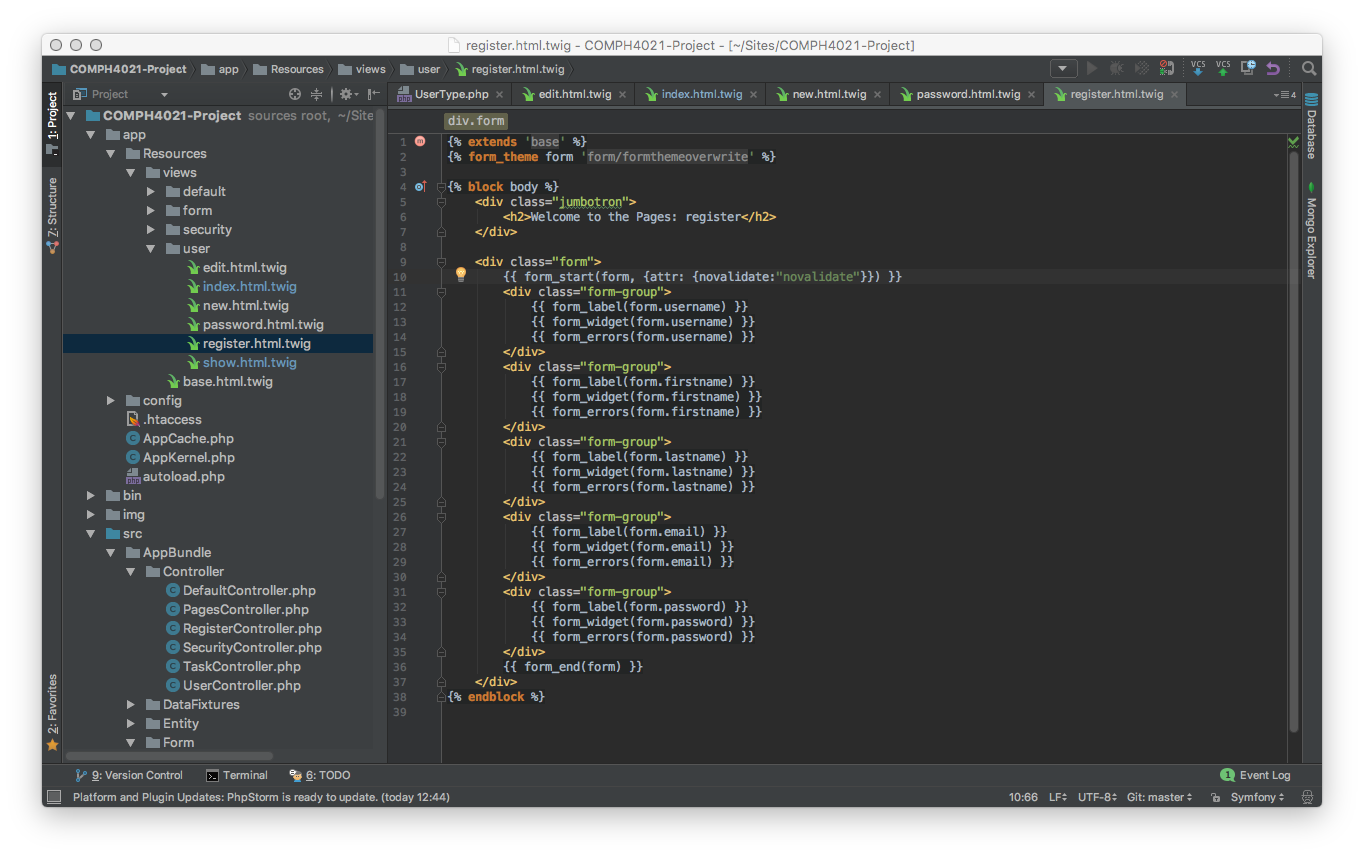
\includegraphics[width=400pt]{figures/form_label.png} % requires the graphicx package
   \caption{Form Label}
   \label{fig:Form Label}
\end{figure}

\section{Validation}

\subsection{Validation of the Forms}

At this stage without populating the form and by using the create button to create a new user in the form there was HTML5 validation. A notification message would pop up with an instruction such as, "Please fill out this field." In order to validate the form or objects on the server side. The form validation needs to be turned off. Figure \ref{fig:Form Validation} shows how this was done.

\begin{figure}[htbp]
   \centering
   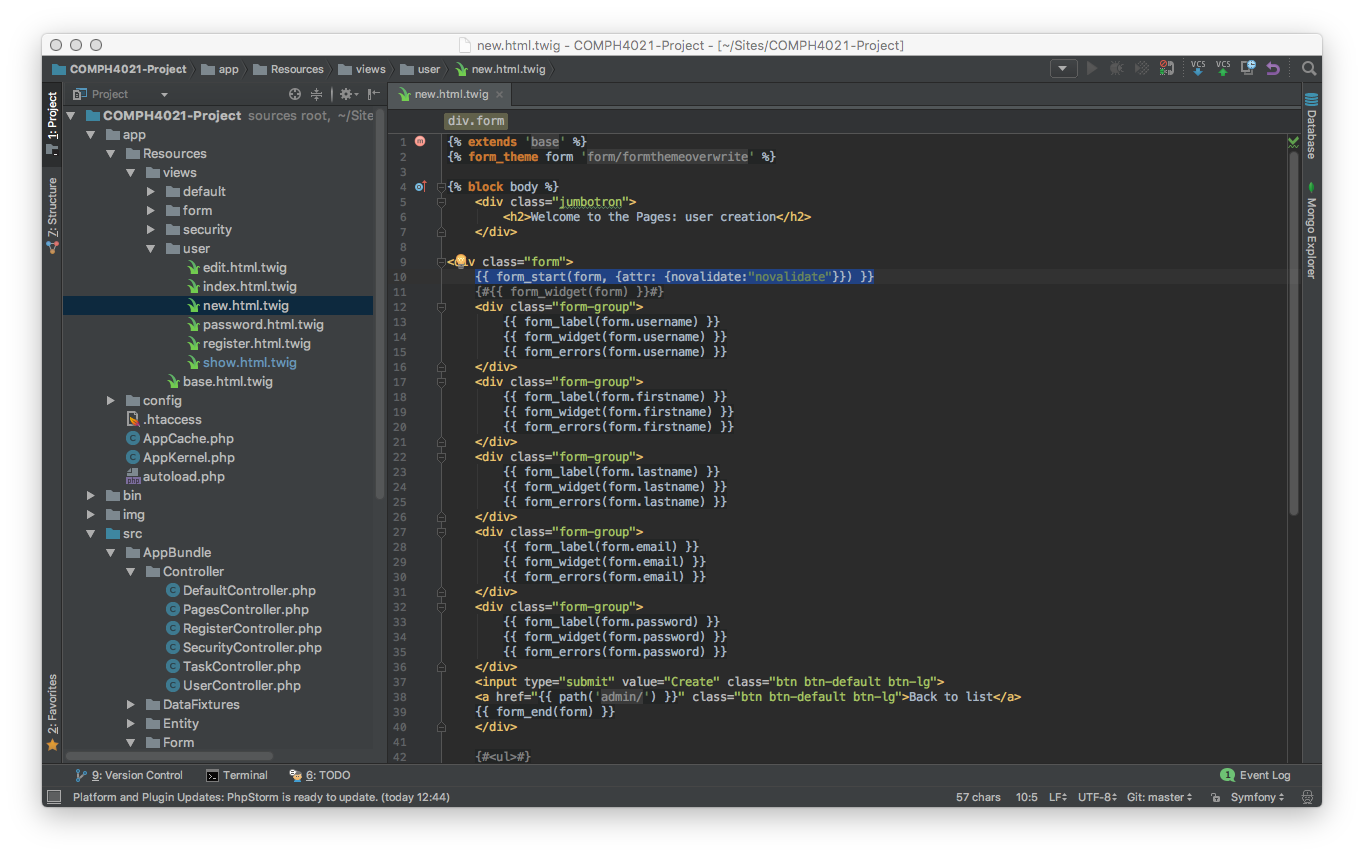
\includegraphics[width=400pt]{figures/form_validation.png} % requires the graphicx package
   \caption{Form Validation}
   \label{fig:Form Validation}
\end{figure}

Line 10 is being passed an instance of the FormType in the form start method. Adding arguments to that such as {attr: {novalidate:"novalidate"}}. With this attribute added there was no server validation. This was performed on the object which is the entity User.php class by adding a use statement such as in line 7 of figure \ref{fig:Entity Validation}. 

\begin{figure}[htbp]
   \centering
   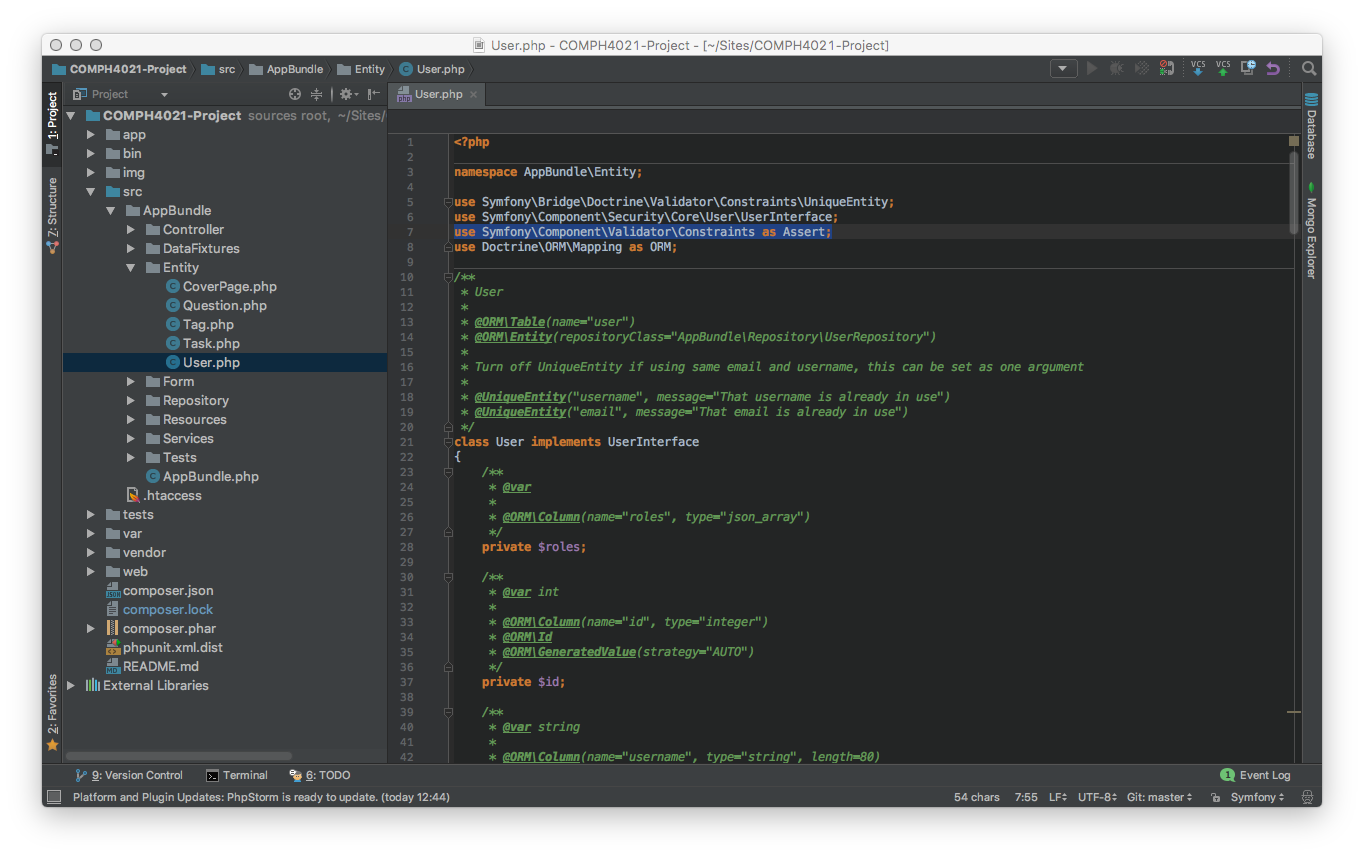
\includegraphics[width=400pt]{figures/entity_validation.png} % requires the graphicx package
   \caption{Entity Validation}
   \label{fig:Entity Validation}
\end{figure}


A use statement in Symfony is a class. With the use statement added it was possible to assert constraints on top of the properties for each of the form fields with reference to figure \ref{fig:Constraints}.

\begin{figure}[htbp]
   \centering
   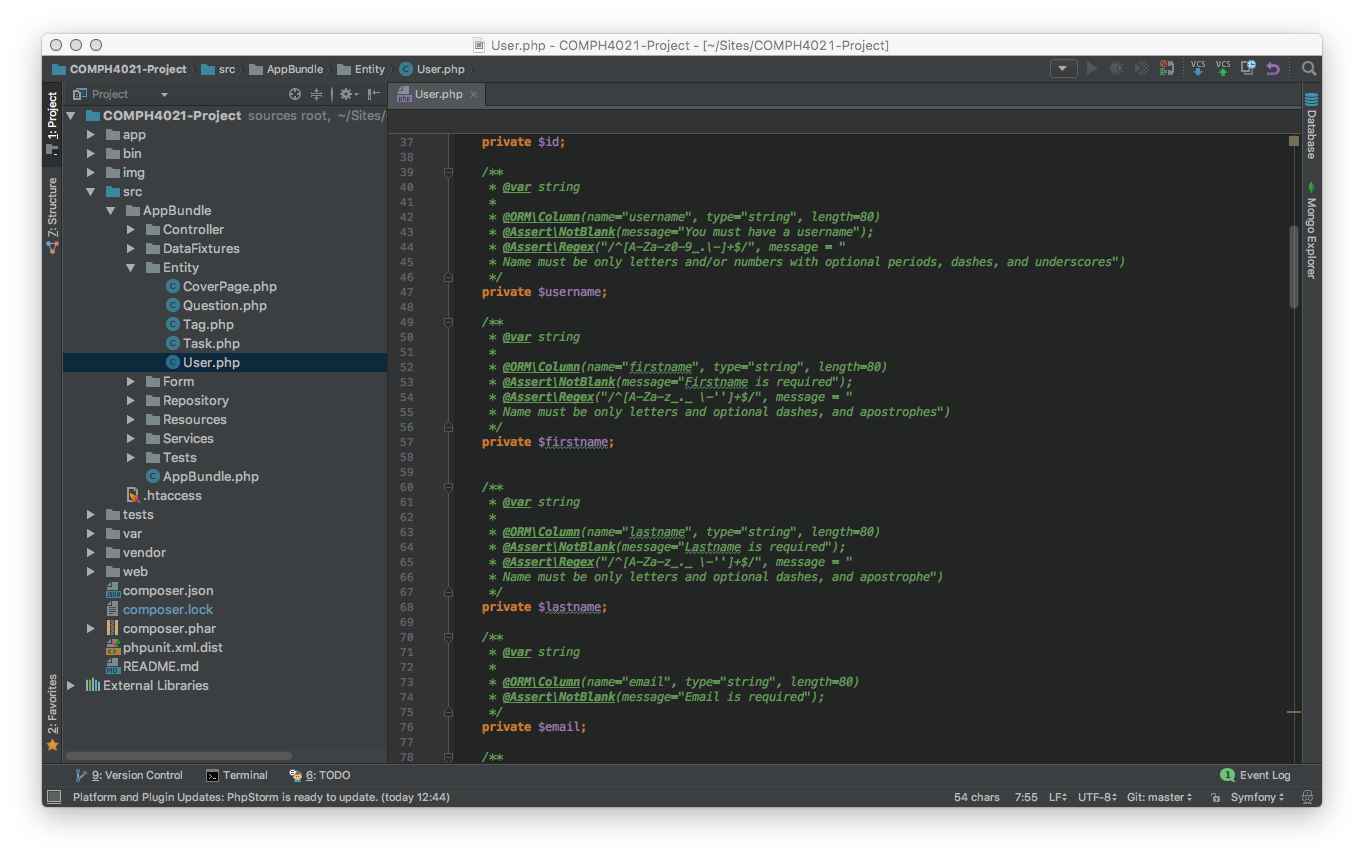
\includegraphics[width=400pt]{figures/assert_constraints.png} % requires the graphicx package
   \caption{Constraints}
   \label{fig:Constraints}
\end{figure}

Functional testing was done at this point in order to make sure everything worked. Another feature which was added was having a unique username and a unique email. This was achieved with yet another use statement which can be found in line 5 of figure \ref{fig:Entity Validation}. In the class declaration there are two arguments passed for each property in line 18 and line 19. The property name that needs to be checked against uniqueness. And a message was also passed in, incase the test failed. The same was created for username. It is possible to set both the username and the email as double arguments for one unique entity call however, this will allow the uniqueness of the email to get through as long as the uniqueness of the username is not there. This is why they were passed in separately. Functional testing was performed in order to confirm the changes which were made worked appropriately.

\section{Theming}

\subsection{Form Theming}

Form theming is a concept which made all the forms look appealing such as the error messages and buttons. Things to remember are, never to adjust the core of Symfony. Instead it is overridden by doing things like telling Symfony where things are that need to be overridden. To proceed with this the error code can be found in the core of Symfony. Figure \ref{fig:Form Errors} shows the error message which was overridden.

\begin{figure}[htbp]
   \centering
   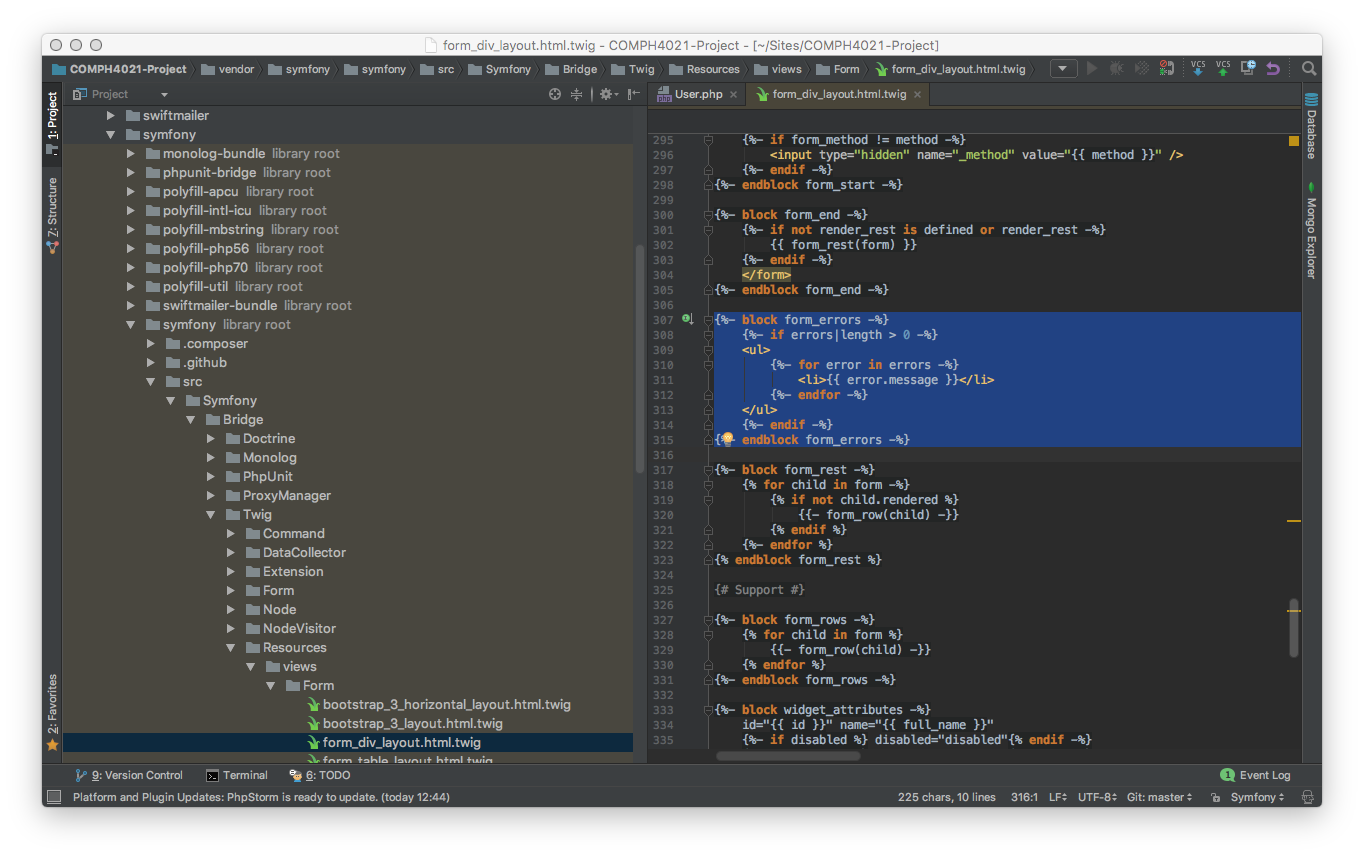
\includegraphics[width=400pt]{figures/form_errors.png} % requires the graphicx package
   \caption{Form Errors}
   \label{fig:Form Errors}
\end{figure}

It was overridden in the Twig template figure \ref{fig:Form Theming} with a Bootstrap dismissible alert placed inside the Symfony error message. The files which use this Twig template are:

\begin{itemize}
  \item edit.html.twig
    \item new.html.twig
      \item password.html.twig
        \item register.html.twig
\end{itemize}

\begin{figure}[htbp]
   \centering
   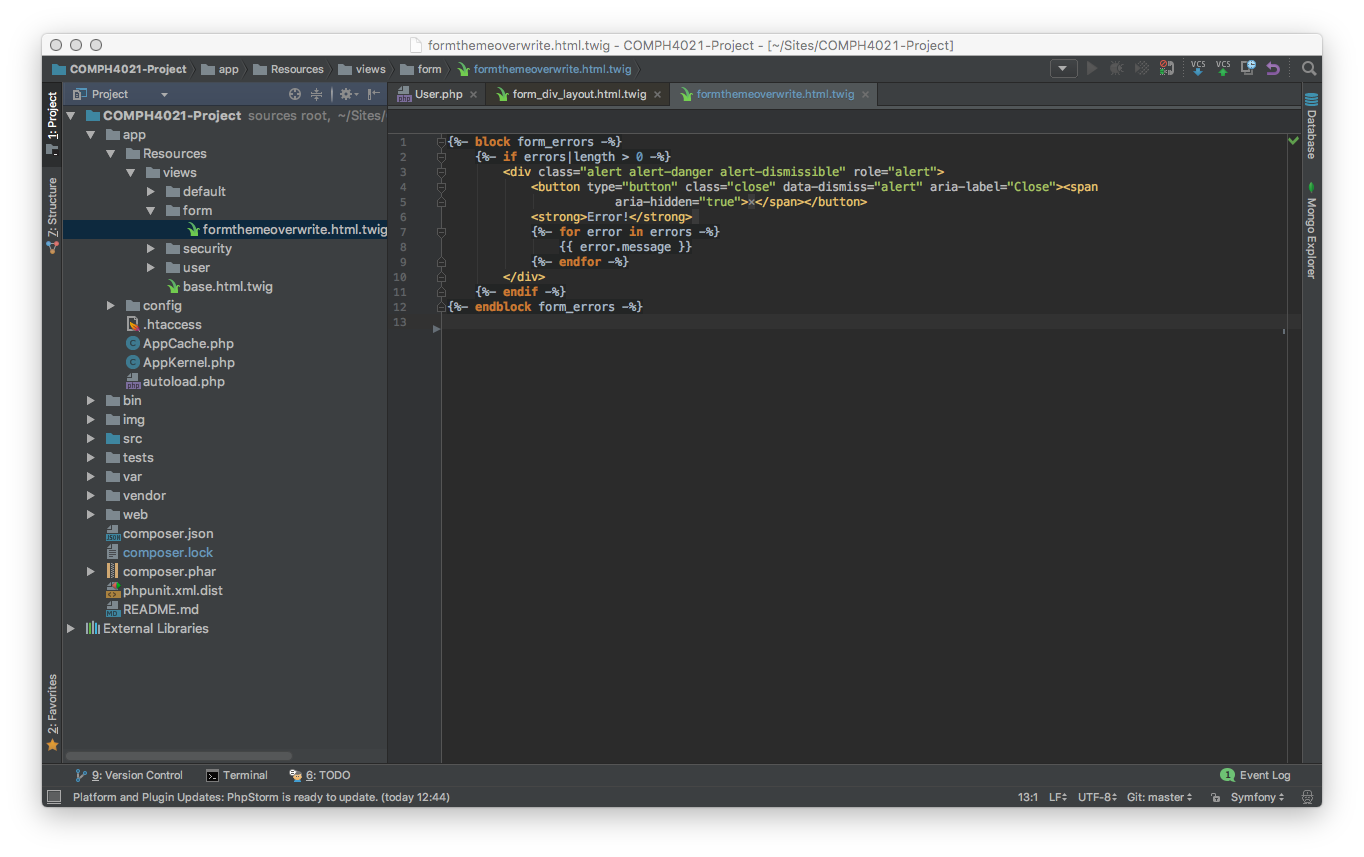
\includegraphics[width=400pt]{figures/formthemeoverwrite.png} % requires the graphicx package
   \caption{Form Theming}
   \label{fig:Form Theming}
\end{figure}

\begin{figure}[htbp]
   \centering
   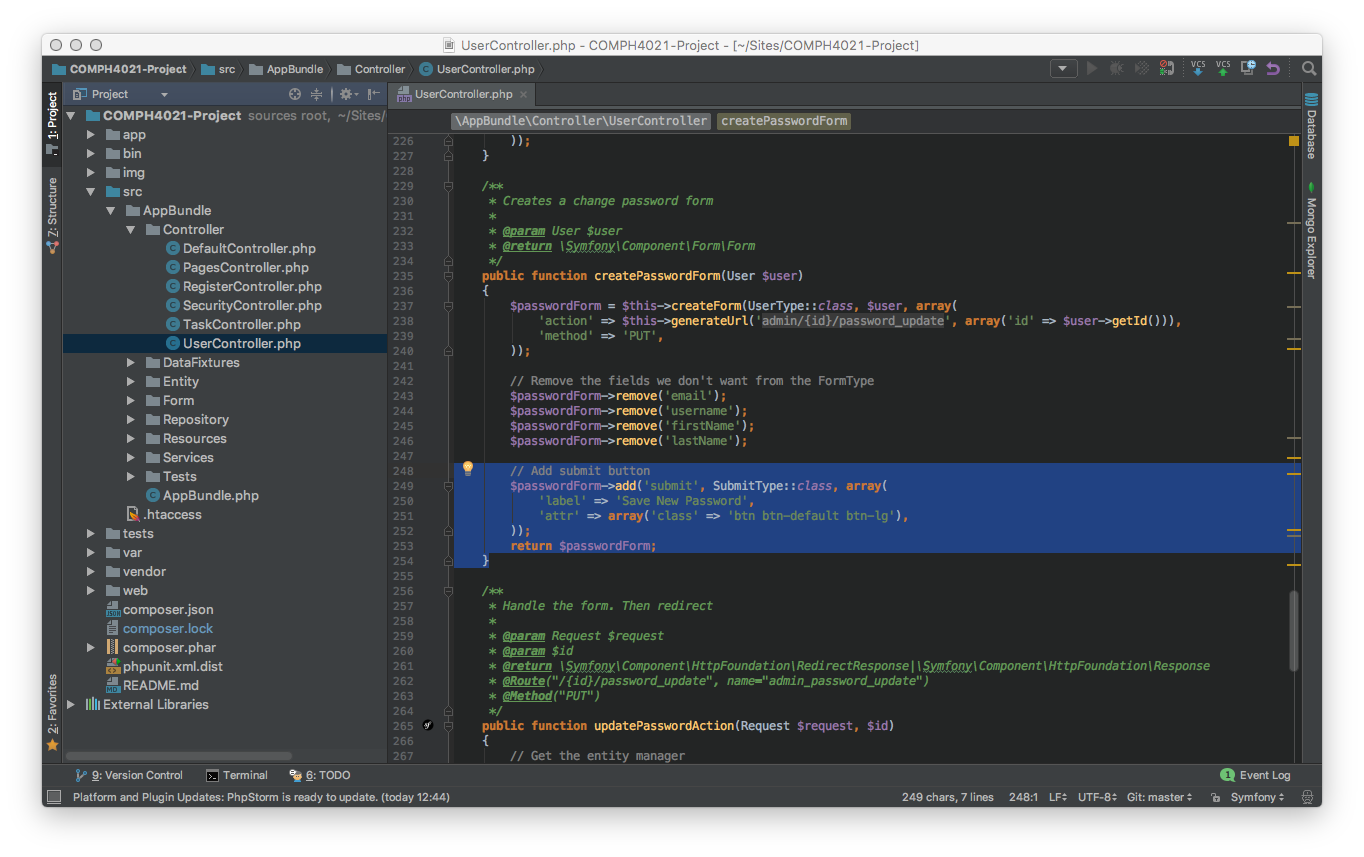
\includegraphics[width=400pt]{figures/usercontroller_button.png} % requires the graphicx package
   \caption{Button Theming}
   \label{fig:Button Theming}
\end{figure}

The buttons were given their own theming and implemented as follow in figure \ref{fig:Button Theming}.

\begin{figure}[htbp]
   \centering
   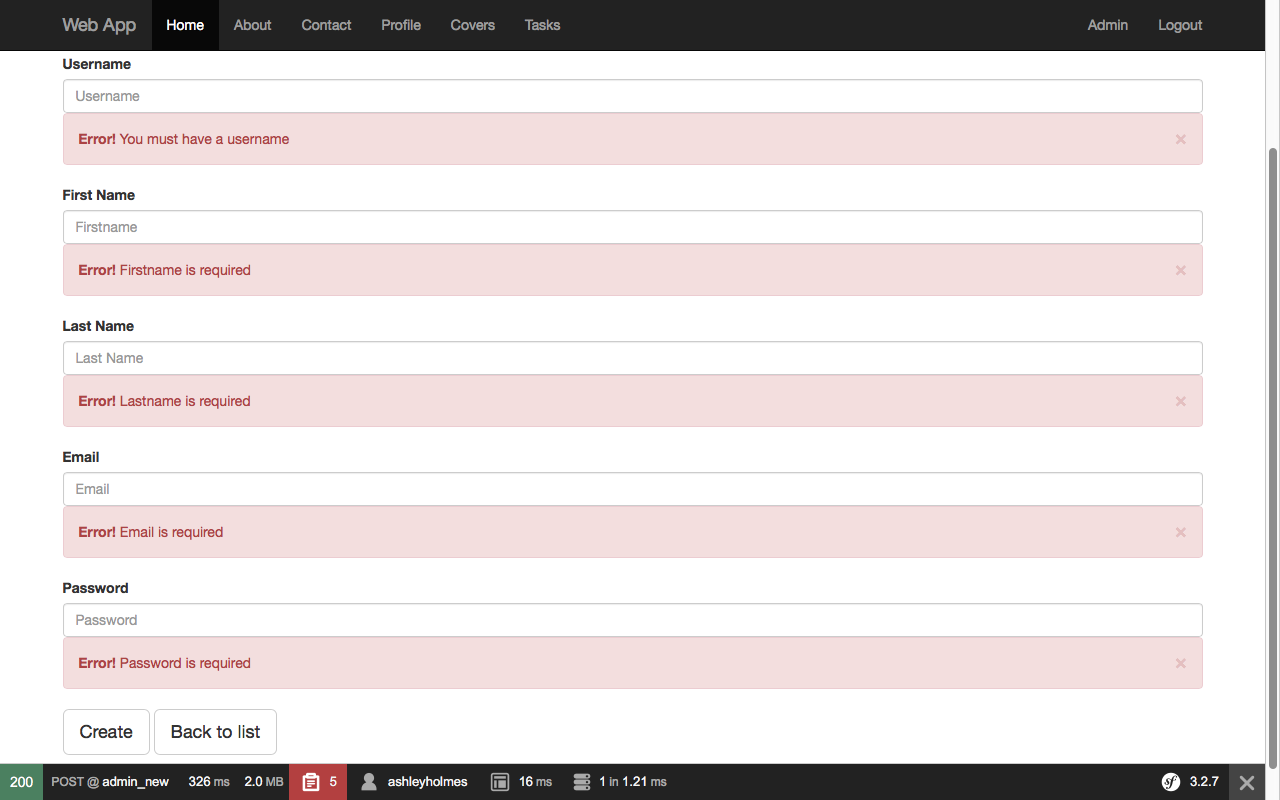
\includegraphics[width=400pt]{figures/form_theming.png} % requires the graphicx package
   \caption{Form Theming Result}
   \label{fig:Form Theming Result}
\end{figure}

\section{Fixtures}

\subsection{Fixtures with Faker}

Fixtures are used to add data into a database in a controlled manner for the purpose of testing or for the initial data which is required for the application to run. The four actions which were necessary for this was as follows:

\begin{itemize}
  \item Use Composer to download the appropriate dependencies.
    \item Adjust the AppKernel.php to use the dependencies.
      \item Write the fixture.
        \item Use the fixture in the console.
\end{itemize}

Every good application needs some way to test the data which is being worked on. This is why fixtures is a good place to start. Before this can be done Composer needs to be installed on the computer and it needs to be installed globally. Instructions for this can be found on the Symfony website. Composer is a dependency manager and it is used to require a bundle from Packagist. Packagist is the main Composer repository. It links packages with Composer and shows Composer where to get the code from. With that completed a terminal command may be issued: composer require --dev doctrine/doctrine-fixtures-bundle with reference to figure \ref{fig:Fixtures}.

\begin{figure}[htbp]
   \centering
   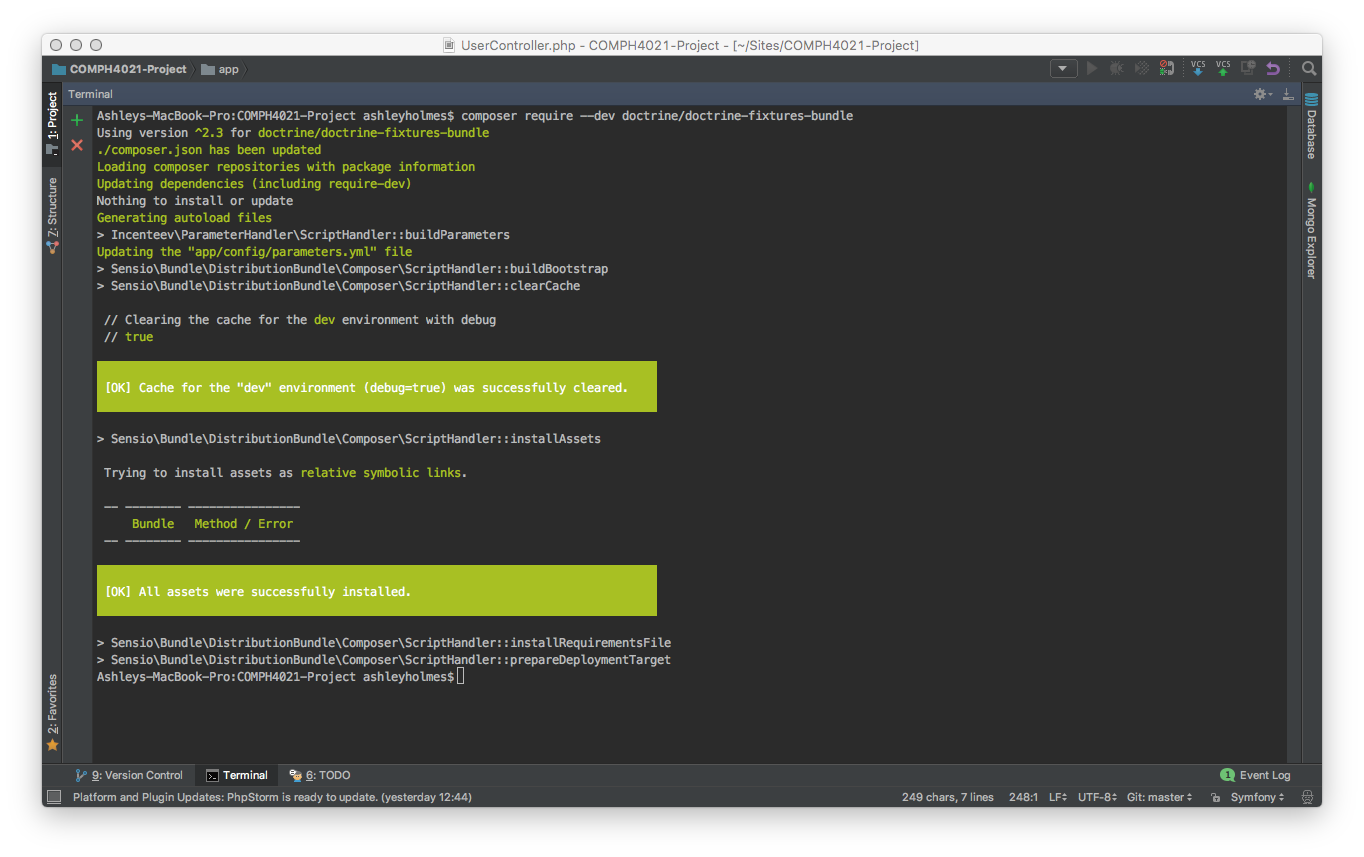
\includegraphics[width=400pt]{figures/fixtures.png} % requires the graphicx package
   \caption{Fixtures}
   \label{fig:Fixtures}
\end{figure}

\begin{figure}[htbp]
   \centering
   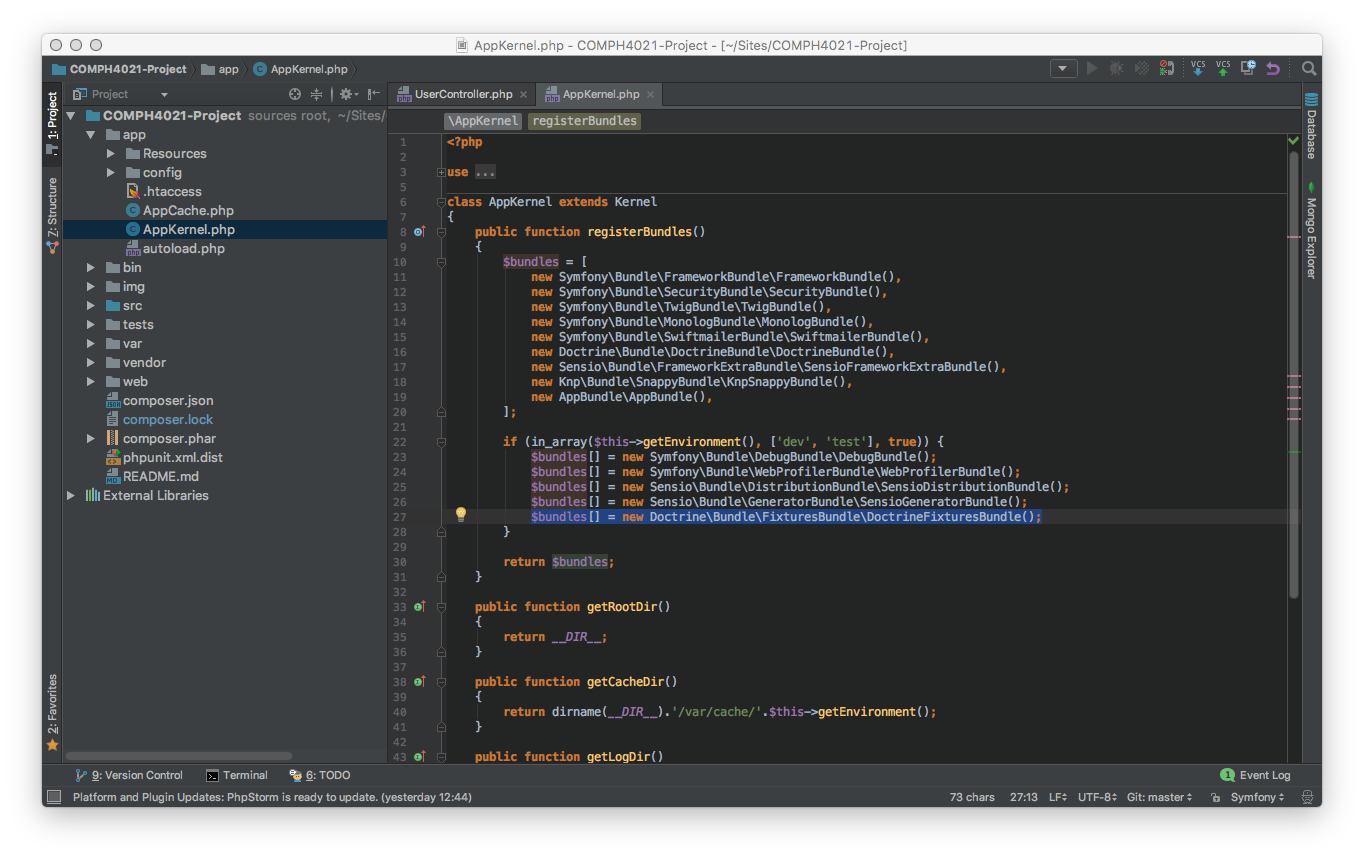
\includegraphics[width=400pt]{figures/bundles.png} % requires the graphicx package
   \caption{Bundles}
   \label{fig:Bundles}
\end{figure}

The following line of code figure \ref{fig:Bundles} was added to AppKernel in the bundles array of which activates the bundle. It was now possible to build a load in fixtures class. In AppBundle a directory is created with the name	 DataFixtures and a class called \newline PopulateUserTable.php. In figure \ref{fig:Faker}

\begin{figure}[htbp]
   \centering
   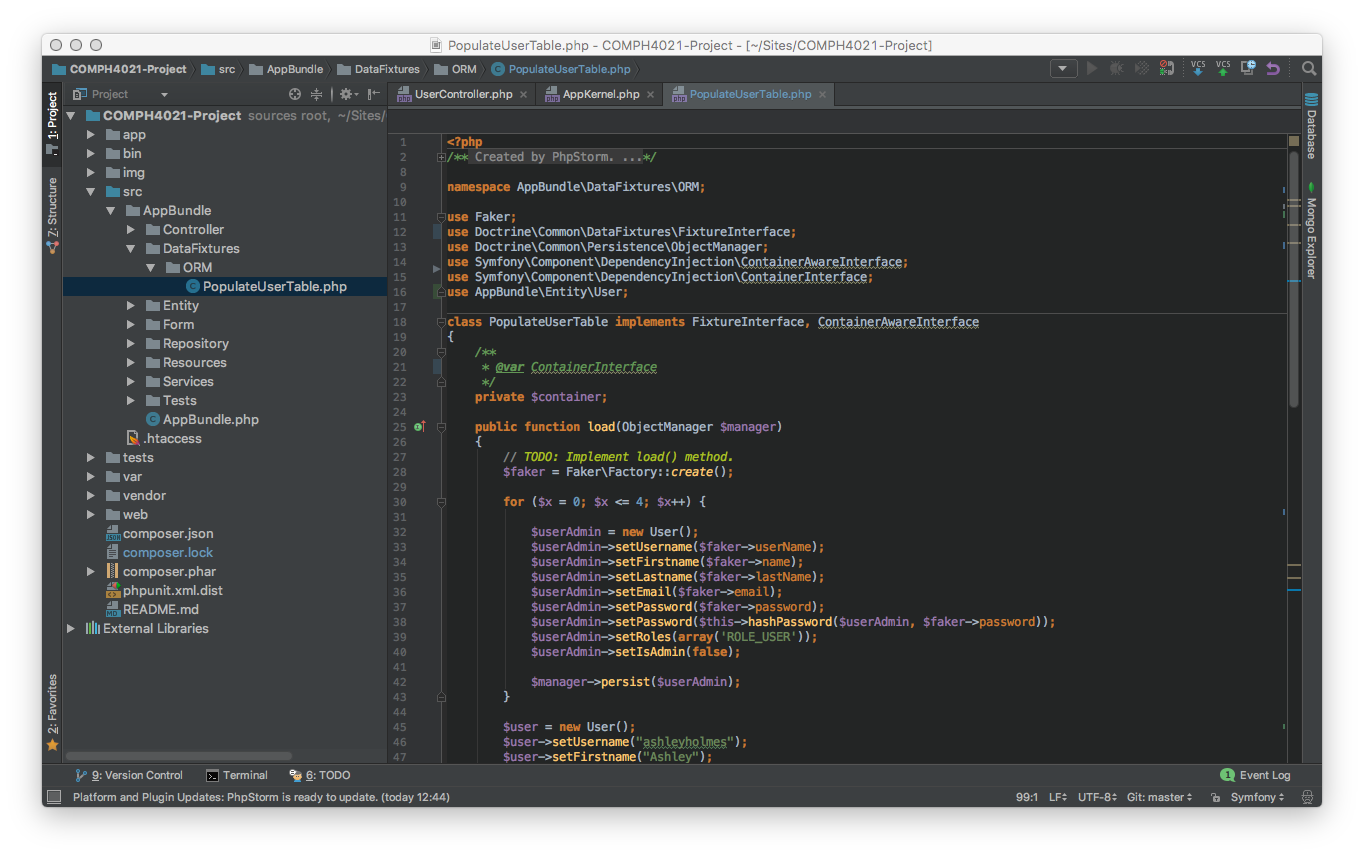
\includegraphics[width=400pt]{figures/faker.png} % requires the graphicx package
   \caption{Faker}
   \label{fig:Faker}
\end{figure}

on line 9 there is a namespace for the file which is also a bundle much like a directory.  It becomes a bundle when a bundle class is added to it. Adding a namespace to a class is organising files from one directory, into a sub directories. The PopulateUserTable class lives in a directory called ORM which lives in a directory called DataFixtures which lives in AppBundle. Which is essentially a folder hierarchy. Each one will be unique as each class name is different. Use statements are included from line 11 to line 16. The one on line 15 has a method which is required as it implements the FixtureInterface. Line 13 is the ObjectManager which enables the manipulation of the EntityManager in order to persist the object to the database which is the use statement in line 12. Line 25 has a public function called load and is what is required by the FixtureInterface and will bring in the object to the function which is also called dependancy injection. Line 11 is the Faker use statement. This is a PHP Library which generates fake data and can be seen in the admin index page. Line 42 shows how the ObjectManager persists it to the User object and line 69 in figure \ref{fig:Object Manager Flush} which writes the data to the database.

\begin{figure}[htbp]
   \centering
   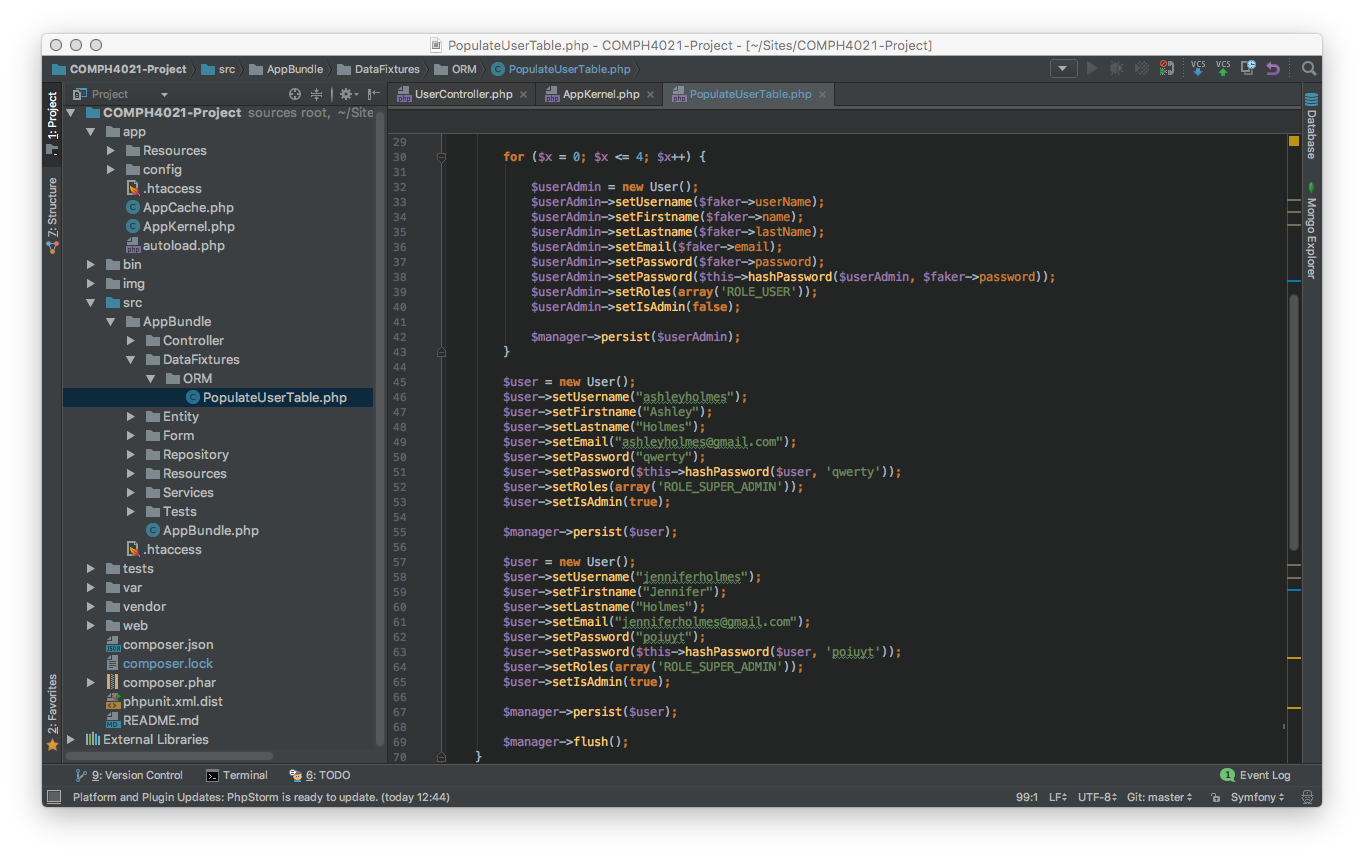
\includegraphics[width=400pt]{figures/objectmanager_flush.png} % requires the graphicx package
   \caption{Object Manager Flush}
   \label{fig:Object Manager Flush}
\end{figure}

\begin{figure}[htbp]
   \centering
   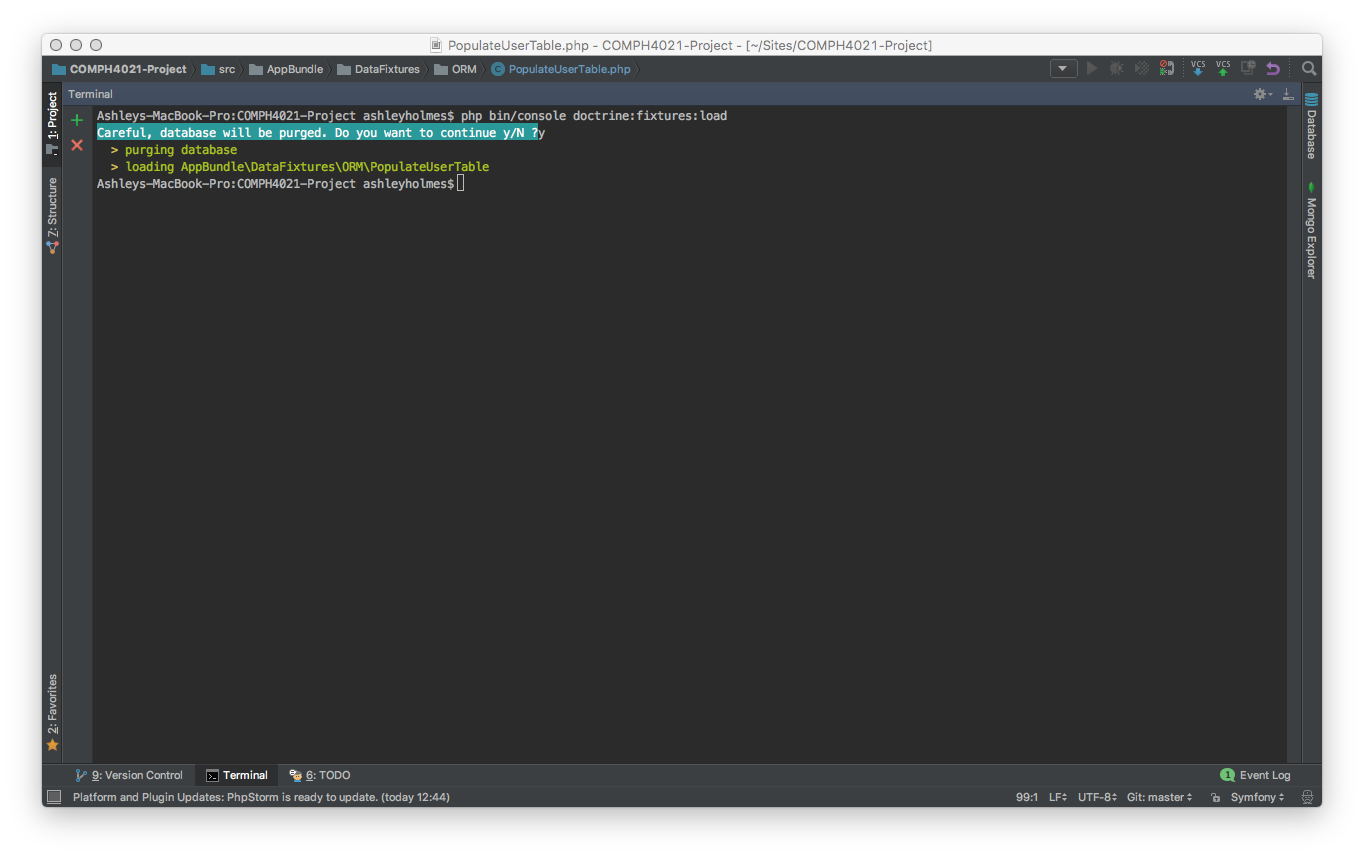
\includegraphics[width=400pt]{figures/fixtures_load_purge.png} % requires the graphicx package
   \caption{Purge Database}
   \label{fig:Purge Database}
\end{figure}

The line in the console window is what is used to purge what is currently in the database and add new data to it. Each user is persisted separately.

\section{Passwords}

\subsection{Password Fixtures}

This section covers passwords and all that was done to encode them. There is a place where to make passwords and there is also a place in the fixtures where users are inherently uploaded. The first thing which was done was to work on the fixtures. There were a few things to do to make that work.

\begin{itemize}
  \item Make the fixture ContainerAware by means of the ContainerAwareInterface.
    \item Adjust the security.yml file with the bcrypt encoder.
      \item Write a method which uses the bcrypt to hash the password.
        \item Encode the passwords in the fixture.
\end{itemize}

When the ContainerAwareInterface was implemented in the class declaration all of the services are then made available for use. This is needed to encode the password in the fixtures file. The file needs to be made ContainerAware. The encoder was added to the security.yml which is figure \ref{fig:Security.yml} lines 4 and 5.

\begin{figure}[htbp]
   \centering
   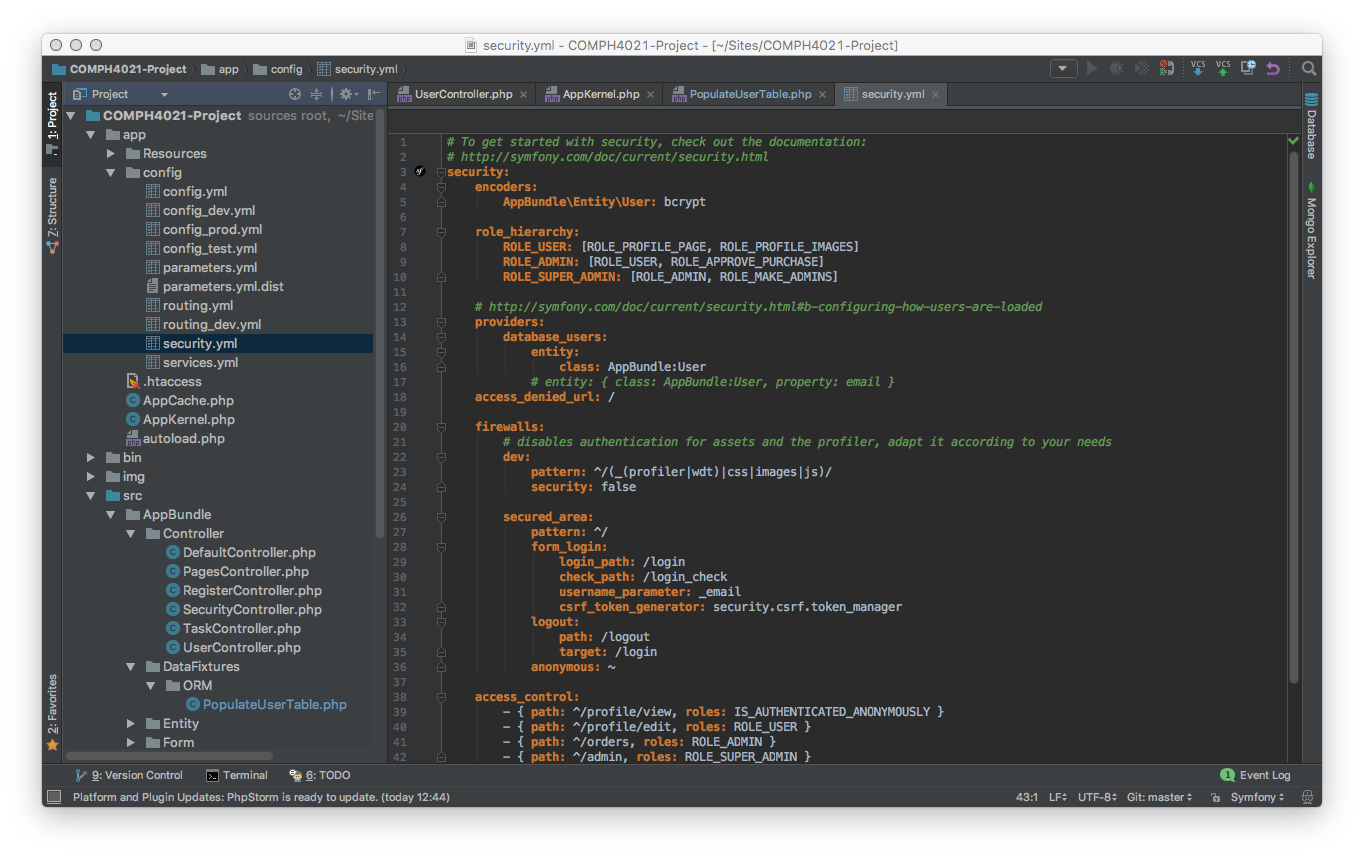
\includegraphics[width=400pt]{figures/security_yml.png} % requires the graphicx package
   \caption{Security.yml}
   \label{fig:Security.yml}
\end{figure}

With that being done bcrypt was available for use. Use statements were also needed to make it work which needed to be added to the PopulateUserTable.php class. The use statements can be found on lines 14 and 16 of figure \ref{fig:Faker} and a private property called container was added in line 23. There is also a public function called setContainer which takes an argument of ContainerInterface and initially sets the container variable to null. Followed by this is a function which does the password encryption in figure \ref{fig:Hash Password}.

\begin{figure}[htbp]
   \centering
   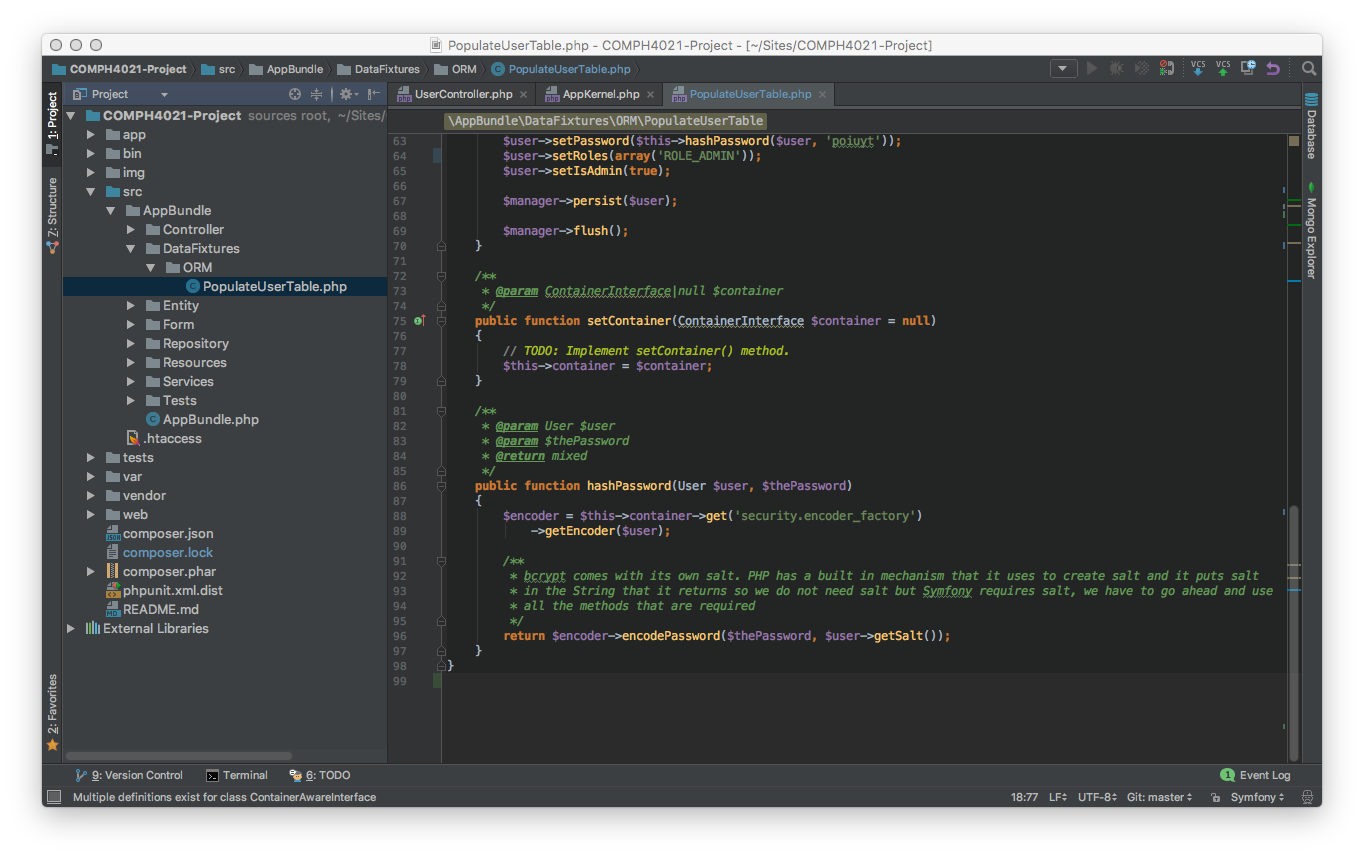
\includegraphics[width=400pt]{figures/hash_password.png} % requires the graphicx package
   \caption{Hash Password}
   \label{fig:Hash Password}
\end{figure}

The entity gets passed into the hashPassword method and the password which needed to be encrypted. With the fixture being containerAware it can be used to get the password encoder from the inbuilt security service. The security service was enabled in the security.yml file and specified which encryption method which was used. Line 88 is where the encoder variable name is to store that object or service. The service is then captured by calling the containers get method and passing in the service which is to be used. In this case, it is the security encoder factory. That service has a method called getEncoder and the entity is passed in once the method is invoked. The object which has been specified encoder has a method called encodePassword and if passed a password and salt to encode it and it will return and encrypted password. The salt to use also needs to be defined however, bcrypt comes with its own salt, PHP has a built-in mechanism which it uses to create salt and it puts the salt in the string which it returns. So salt is not needed however, it is required by Symfony as all the methods need to be used which are required. This is why a getSalt function had to be created in the User entity figure \ref{fig:getSalt Method} and returns null as bcrypt does not require anything.

\begin{figure}[htbp]
   \centering
   \includegraphics[width=400pt]{figures/salt.png} % requires the graphicx package
   \caption{getSalt Method}
   \label{fig:getSalt Method}
\end{figure}

Encoding the password is executed in line 38 of figure \ref{fig:Object Manager Flush} by capturing the hashPassword method which was created and passing in the user object and the String of the password. The encrypted passwords are in figure \ref{fig:Password}

\begin{figure}[htbp]
   \centering
   \includegraphics[width=400pt]{figures/password.png} % requires the graphicx package
   \caption{Password}
   \label{fig:Password}
\end{figure}

\subsection{Password Services}

The last section covered encoding passwords from a fixture. This section is oriented around encoding passwords from a controller and writing the service. To do this, the following steps are needed:

\begin{itemize}
  \item Implement the UserInterface.
    \item Create the service for encoding the passwords.
      \item In the sevices.yml file implement the service.
        \item Use the service container to call the encoding method.
\end{itemize}

\begin{figure}[htbp]
   \centering
   \includegraphics[width=400pt]{figures/user_interface.png} % requires the graphicx package
   \caption{UserInterface}
   \label{fig:UserInterface}
\end{figure}

Symfony is a set of bundle which does what it is asked to do. It is possible to create a security system from scratch if that is what was intended. However, Symfonys in-built system is so robust. Using it saved much coding time and gave much more features than it would be possible to code from the bottom up. To use Symfonys security system the UserInterface needed to be implemented. From the documentation. The UserInterface has five different methods to implement figure \ref{fig:UserInterface} shows this.

To implement these methods a statement was added to the User entity class. From figure \ref{fig:Entity Validation} which we originally shown in the validation section of this chapter. Line 6 is added and the interface is implemented on line 21. Some of the methods were already in the User entity class. Only the ones which are not already there were added. Such as a function by the name of eraseCredentials which was left blank. Although it is not used in this application. The class is required by the interface. The same use statement is added to the service. A service is an object whose responsibility is to perform a specific task. The service which was created was to encrypt the password. Services are a three step process.

\begin{enumerate}
  \item Create the service.
    \item Enable the service in the services.yml file.
      \item Use the service in the controller by calling it with the containers get method.
\end{enumerate}

Starting with creating a file called UserManager.php which lives in a folder called Services which was added to AppBundle. This file was namespaced in order to match the hierarchy. And then the use statement from the User entity was added. In addition was this line 11 in figure \ref{fig:UserManager}

\begin{figure}[htbp]
   \centering
   \includegraphics[width=400pt]{figures/user_manager.png} % requires the graphicx package
   \caption{UserManager}
   \label{fig:UserManager}
\end{figure}

The private variable encoderFactory in line 19 is where the encoderFactory is stored. The constructor in line 24 is injected with the encoderFactory object and therefore no setter method was needed. The method that encodes the password is on line 33 and takes two parameters such as the userInterface and a String which represents the password which is to be encrypted. A variable was set in line 38 to store the encoded password and the it needs to be encoded which is done by the EncoderFactory which takes an argument and the UserInterface is passed in. The encodePassword method in line 39 takes two arguments. The String that needs to be encoded and the salt which is used. Which is actually bcrypt. The password was set into the entity by user which implements the UserInterface and by calling the setPassword method pass in the hashedPassword.

The second step was to go into the services.yml file and enable the service. The service was named which could be anything but it was named in order to indicate where it resides. Then tell the caller of the service where the service is on line 8 of figure \ref{fig:Yaml Services}. So providing the namespace of the service which was created. So when the AppBundle, Services, UserManager is called in the controller it will grab this class. Then tell the container what arguments to pass into it. The arguments on line 9 are passed in which is the encoder factory object.

\begin{figure}[htbp]
   \centering
   \includegraphics[width=400pt]{figures/services_yml.png} % requires the graphicx package
   \caption{Yaml Services}
   \label{fig:Yaml Services}
\end{figure}

\begin{figure}[htbp]
   \centering
   \includegraphics[width=400pt]{figures/user_controller.png} % requires the graphicx package
   \caption{UserController}
   \label{fig:UserController}
\end{figure}

In the UserController under the newAction the service needed to be called in and encrypt the password which would be passed. This was done on line 56 of figure \ref{fig:UserController} with the containers get method which was the same name used in the services.yml file. The encoded factory is automatically pulled in as an argument was attached to that class. Line 57 calls the method that was created in the UserManager. Passing the entity which is the user and the password.

\subsection{Change Password Form}

The following is explained in order to create and handle the new password form.

\begin{itemize}
  \item Create a new password.html.twig file.
    \item Create a password controller.
      \item Password form generator method.
        \item Form submission controller.
          \item Redirect.
\end{itemize}

A new file was created in the user directory called password.html.twig as with figure \ref{fig:Password Twig template}.

\begin{figure}[htbp]
   \centering
   \includegraphics[width=400pt]{figures/password_html_twig.png} % requires the graphicx package
   \caption{Password Twig template}
   \label{fig:Password Twig template}
\end{figure}

\begin{figure}[htbp]
   \centering
   \includegraphics[width=400pt]{figures/change_password.png} % requires the graphicx package
   \caption{Change Password Form}
   \label{fig:Change Password Form}
\end{figure}

Creating the controller in the UserController. There were two things to cover in writing the controller which handle the form. Which was create the view and display it. And then handle the form and redirect it which will be covered in a later section.

\begin{figure}[htbp]
   \centering
   \includegraphics[width=400pt]{figures/password_action.png} % requires the graphicx package
   \caption{passwordAction Controller}
   \label{fig:passwordAction Controller}
\end{figure}

The Action suffix is required on line 200 as it is a controller which handles a view. The view is the Twig template. Passing in the id which creates a hook into the entity manager on line 202 using the container. And then using the entity manager to get the data with the repository using the find method and pass it inside the entity object. If the entity is not found and exception would be generated. This happens on line 205 to 209. A route is then added as annotation in line 194 in order to get into this function. The route needs to be passed an id and give it a unique name. In other words a variable id and then password separated by a forward slash. The name in the route is what was used in the Twig template. The next annotation is what method was used to get to the route which is a GET String. The last annotation is Template which does not take an argument as the suffix Action was used. Symfony can figure out where it is in order to get the template. In this case it would look for a password.html.twig within the Resources folder and a folder underneath that called user as that is the name of the controller. The form is then created in line 220 by calling the createPasswordForm method. Lastly, render the view by passing the view the entity and the form in an array on line 223. A link to the route was created in line 61 of figure \ref{fig:show.html.twig} for the user which has access to look at the page can change a password. So far this only displays the form. Once a change was made to the password a way in which to handle the form submission was required. This is shown in figure \ref{fig:createPassword Form} which creates a new form.

\begin{figure}[htbp]
   \centering
   \includegraphics[width=400pt]{figures/create_password_form.png} % requires the graphicx package
   \caption{createPassword Form}
   \label{fig:createPassword Form}
\end{figure}

Line 235 gets passed the entity which is the User.php class and then the form gets returned to the invoker in line 253. The validation is managed in figure \ref{fig:Password Form Validation} on line 288. If the form validates, the data gets added to the database. If not, the rest of the action will execute and return another form with the errors. This is done through annotation. Line 291 is the service which was previously written and encode the password. The password has been encoded and the entity already persisted. In line 294 it is flushed to the database and then redirected to another page which is the admin show page in line 297 which requires an id. Some functional testing was done to ensure all implementations were in order.

\begin{figure}[htbp]
   \centering
   \includegraphics[width=400pt]{figures/create_password_form_validation.png} % requires the graphicx package
   \caption{Password Form Validation}
   \label{fig:Password Form Validation}
\end{figure}

\section{Authentication}

\subsection{Login Form}

Authorisation is about logging a user in. If a user is on the site whether they are logged in or not. They are still authenticated, however the authentication is anonymously as was seen at the bottom of figure \ref{fig:Web Debug Toolbar and Profiler Extended}. This is where the login form is appropriate. To do this is as follows:

\begin{itemize}
  \item Adjust the security.yml.
    \item Implement role hierarchy.
      \item Look at how the security system takes over the login process.
        \item Go through the SecurityController.
          \item Adjust the twig template for login.
\end{itemize}

The five areas where the configurations were set are role hierarchy, providers, firewalls, secured area and access control in figure \ref{fig:Security.yml}. Role hierarchy is the role of the user. With the roles inside of role hierarchy defines the page level or folder level specific actions which the user can do. Role Admin inherits all the roles which the user has in addition to other page or folder level roles. The same for role Super Admin. Providers has database users meaning the roles will come from the database. The providers need to be told where to get the entity from,  since using the database user and this is AppBundle:User and the property to check against is the username. Firewalls is just as it sounds. It gives specific access or meaning to areas of the website. The one on line 22 is for development purposes and it states that there will be no security on any profiling pages. In secured area the pattern was set to anything. Paths were given which would later be used by the SecurityController in AppBundle Controller directory. Anonymous was set to everything in order to allow access to the login page by all. The Symfony documentation provides a sample of the SecurityController which was available for use of which was modified to suit the needs of this project. The controller can be seen in figure \ref{fig:SecurityController}.

\begin{figure}[htbp]
   \centering
   \includegraphics[width=400pt]{figures/security_controller.png} % requires the graphicx package
   \caption{SecurityController}
   \label{fig:SecurityController}
\end{figure}

\begin{figure}[htbp]
   \centering
   \includegraphics[width=400pt]{figures/login_html_twig.png} % requires the graphicx package
   \caption{Login Form}
   \label{fig:Login Form}
\end{figure}

\begin{figure}[htbp]
   \centering
   \includegraphics[width=400pt]{figures/symfony_profiler_login.png} % requires the graphicx package
   \caption{Symfony Login Profiler}
   \label{fig:Symfony Login Profiler}
\end{figure}

\begin{figure}[htbp]
   \centering
   \includegraphics[width=400pt]{figures/access_decision_logs.png} % requires the graphicx package
   \caption{Symfony Login Profiler}
   \label{fig:Symfony Login Profiler}
\end{figure}

A sample login form was also available from the Symfony documentation page of which was used and changed and can be seen in figure \ref{fig:Login Form}.

Once logged in the Symfony debug toolbars profiler page shows which roles belong to the user and these match what was added to the security.yml and used in the SecurityController.

\section{Controllers}

\subsection{Extending the controller}

The login form and controllers were extended to have a successful user experience. The below section covers this.

\begin{itemize}
  \item Make errors look better.
    \item Adjust base template with the proper links.
      \item Make login by email available.
        \item Use twig function for assigned roles.
          \item Using the repository for username or email.
\end{itemize}

As of now the template which was used from the Symfony website was using a translation service, which was commented out in line 10 of figure \ref{fig:Login Form}. This was changed to a Bootstrap error message as used in line 9 to achieve the result in the image below. Adjustments were then made to the base.html.twig file where links such as login and logout were added. Twig logic was also added using its own is granted function to do a check for whether the user was authenticated with the relevant role and if so display the login and logout link at the top of the page. In figure \ref{fig:User Roles in the the base template} this can be seen from line 54 to 69.

\begin{figure}[htbp]
   \centering
   \includegraphics[width=400pt]{figures/login_error.png} % requires the graphicx package
   \caption{Login Form Error}
   \label{fig:Login Form Error}
\end{figure}

Line 39 of the security.yml shows how to achieve a login through email. On line 24 the input tag for the label in the login.html.twig was change to accept the email instead of username to make the change which was done in the YAML file. In order to login with both username and email address an extra step was needed. The code for this was picked up from Symfony documentation page and placed in the UserRepository figure \ref{fig:UserRepository}.

\begin{figure}[htbp]
   \centering
   \includegraphics[width=400pt]{figures/base_html_twig.png} % requires the graphicx package
   \caption{User Roles in the the base template}
   \label{fig:User Roles in the the base template}
\end{figure}

\begin{figure}[htbp]
   \centering
   \includegraphics[width=400pt]{figures/user_repository.png} % requires the graphicx package
   \caption{UserRepository}
   \label{fig:UserRepository}
\end{figure}

\section{Roles}

\subsection{Putting roles in the database}

Roles are placed into the database and interacted with through the Twig templates and controllers. Below is how it was done.

\begin{itemize}
  \item Add a property in order to use JSON array type.
    \item Update the schema.
      \item Set role by making adjustments in the controllers.
        \item Adjust the fixtures.
\end{itemize}

So far the getRoles method has been used as with the UserInterface. However, there has been no mechanism to store values. To store values, a private property was addd to the User.php class in line 28 of figure \ref{fig:JSON array} with the JSON array annotation above it. A getter was already in place. Only a setter method needed to be added. The setter method would be passed in an array of roles. Once this was complete the schema was updated through the command line.

\begin{figure}[htbp]
   \centering
   \includegraphics[width=400pt]{figures/json_array.png} % requires the graphicx package
   \caption{JSON array}
   \label{fig:JSON array}
\end{figure}

At the initial creation of every user. That user was assigned the role of user by adding the two lines of code in the UserController. Line 64 and 65 show this with reference to figure \ref{fig:UserController}. In PopulateUserTable the fixtures were also adjusted to add the roles to the users which were created. Back in figure \ref{fig:Object Manager Flush} it was possible to see.

\subsection{Using the roles in the database}

This section covers how to use the roles from a database.

\begin{itemize}
  \item Make User Admins from Super Admins.
    \item Adjust the fixture to reflect this.
\end{itemize}

Making the user an Admin involved creating a private property in User.php called isAdmin of type boolean. As there is no boolean in SQL, instead this was replaced with a TINYINT of one or a zero using annotation in line 89 of figure \ref{fig:isAdmin}. A getter and a setter were also created for this attribute.

\begin{figure}[htbp]
   \centering
   \includegraphics[width=400pt]{figures/is_admin.png} % requires the graphicx package
   \caption{isAdmin}
   \label{fig:isAdmin}
\end{figure}

The schema had to be updated after this, in order to update the database with the changes which were made and add the new column. A checkbox was then added to the view in figure \ref{fig:CheckboxType} lines 60 to 63, in order for the super user to add the role of Admin. 

\begin{figure}[htbp]
   \centering
   \includegraphics[width=400pt]{figures/checkbox_type.png} % requires the graphicx package
   \caption{CheckboxType}
   \label{fig:CheckboxType}
\end{figure}

The logic for this was placed inside the UserController.php in the newAction function on line 59. The isAdmin was also set to true for both the Super Admin and the Admin with exclusion to the regular users in the PopulateUserTable.php 

\section{Authorisation}

\subsection{Access Control}

\begin{itemize}
  \item Access control in security.yml.
    \item Access denied parameters.
\end{itemize}

In the section of authentication. The access control attribute was left empty. In this section it will be completed. Creating the control list asserts the type of role to have access to a set of pages. It is available to see at the bottom of the security.yml file \ref{fig:Security.yml}. It is a hierarchy for users to view specific pages. On line 18 there is an access denied url and this will send an any user back to the home page incase they are denied something which only works for authenticated users and not anonymous users.

\section{CSRF Protection}

\subsection{Testing the roles}

By generating a few controllers to demonstrate some of the access control configurations and protecting agains Cross-Site Request Forgery attacks.

\begin{itemize}
  \item Generate a controller in console.
    \item Adjust the generated twig files.
      \item Adjust base file.
        \item Test against ACL.
          \item Add CSRF.
\end{itemize}

Making a controller class in the terminal requires the following command statement, php bin/console generate:controller. Giving it the name AppBundle:Pages, with a routing format of annotation and using a template format. Then by giving the name of the controllers which is preferred to have inside the controller class. The first was called Contact which needed to be appended with the name Action as a suffix. A second is created for Profile. The third for About and the last for Covers and Tasks. By confirming the generation, Symfony creates all the necessary files. The Twig templates were then adjusted to suit as the paths to the newly generated pages needed to be added. With that in place the menu has now been updated. And the navigation works between all pages which are all publicly accessible. When logging in with Super Admin privileges the Covers and Tasks tab is available for view. To add the CSRF protection. This was simply in line 32 in the security.yml and then adding a token in the login.html.twig template. The token is on line 41 and 42 of figure \ref{fig:CSRF Token}. The token is available to view using inspect element in the browser in figure 

\begin{figure}[htbp]
   \centering
   \includegraphics[width=400pt]{figures/csrf_token.png} % requires the graphicx package
   \caption{CSRF Token}
   \label{fig:CSRF Token}
\end{figure}

\begin{figure}[htbp]
   \centering
   \includegraphics[width=400pt]{figures/csrf_token_element.png} % requires the graphicx package
   \caption{CSRF Token Browser}
   \label{fig:CSRF Token Browser}
\end{figure}

\subsection{Controller and templates adjustments based on user roles}

Controllers and templates are adjusted based on the roles which are stored in the database and which are stored in the entity of the users which are viewed.

\begin{itemize}
  \item Restrict Super Admins from editing same Admin.
    \item Flash messages preventing confusion.
      \item Remove links for editing other Admins.
\end{itemize}

At this stage when logging in with the role of Super Admin it was possible for one Super Admin to edit the profile or password of another Super Admin. This needed to be prevented. In the editAction of the UserController a check was implemented in order to check if the user which is in the entity. Not the currently logged in but the entity which is viewed on the user list. There will be a check to verify if that user has the role of Super Admin or not. If they are a user then the authenticated user will be directed back to another page. This can be directly checked in array function on line 103 of figure \ref{fig:editAction}. Looking for the role ROLE SUPER ADMIN and calling the getRoles method which returns an array. If that role was inside the entity which was being viewed then the user would be returned to the show page. With not being able to go into and edit another users edit page. That user was not able to see if anything was happening behind the scenes. Therefore a message was to be created to tell the user what was happening. Symfony has an in-built session management system. Within that system is what is called flash messages which is on line 106. Chained onto that is the add method which takes two arguments. The first is the name of the flash message and the message to the user. These flashbag messages are displayed in the show.html.twig template. Figure \ref{fig:Show Page} has these for view on lines 8 and 16. This was also needed in the function passwordAction and deleteAction. A better approach to this was to not present those links to the user at all. So the adjustment was made and is on line 55 to 59 by means of an if statement in figure \ref{fig:User not in ROLES}. It was also necessary to add this to the index.html.twig.

\begin{figure}[htbp]
   \centering
   \includegraphics[width=400pt]{figures/edit_action.png} % requires the graphicx package
   \caption{editAction}
   \label{fig:editAction}
\end{figure}

\begin{figure}[htbp]
   \centering
   \includegraphics[width=400pt]{figures/show_page.png} % requires the graphicx package
   \caption{Show Page}
   \label{fig:Show Page}
\end{figure}

\begin{figure}[htbp]
   \centering
   \includegraphics[width=400pt]{figures/user_not_in_roles.png} % requires the graphicx package
   \caption{User not in ROLES}
   \label{fig:User not in ROLES}
\end{figure}

\section{Registration}

\subsection{Registration Controller}

The RegisterController was associated with creating an action which creates a form. Displays it and processes the form for a new user.

\begin{itemize}
  \item Create RegisterController.
    \item Create a new register template.
      \item Add flashbag messages.
\end{itemize}

\begin{figure}[htbp]
   \centering
   \includegraphics[width=400pt]{figures/register_controller.png} % requires the graphicx package
   \caption{RegisterController}
   \label{fig:RegisterController}
\end{figure}

Using the entity of type user. A variable of type form was created. Inside that variable a createForm object was placed. It uses the new UserType and the entity which the form was created from. For this form the isAdmin was removed as it was not needed. And a button created for the submission. This is not using the template object so what needs to be returned is a rendering statement as this render. Placed inside is the template which it will be using which is the argument. In this case it was the register template. An array was added and this is where the objects are passed to the response object which creates the view. The entity is passed into the array and then the form. A route is then defined as annotation using @Route /register. Another annotation needed was the @Template to tell that annotation which twig file it will be rendering from.

\begin{figure}[htbp]
   \centering
   \includegraphics[width=400pt]{figures/register_html_twig.png} % requires the graphicx package
   \caption{Register Twig Template}
   \label{fig:Register Twig Template}
\end{figure}

The register template is very similar in code to the new user creation form. This form request needed to be handled. It was achieved by whats on line 33 of figure \ref{fig:RegisterController}. Then do a check to see if the form was posted and if it was valid. If the form was posted and was not valid there needed to be a redirect to the same place in order to be rendered with mistakes which come in the entity.

\begin{figure}[htbp]
   \centering
   \includegraphics[width=400pt]{figures/register_errors.png} % requires the graphicx package
   \caption{Register with Errors}
   \label{fig:Register with Errors}
\end{figure}

When handling the form incase it was valid. There were a couple of values which needed to be explicitly set as it was not handled by the FormType. The password needed to be encoded. And set ROLE USER inside the set roles method and that needed to be of type array. And call the setAdmin method and called it false as the new user was not able to be made admin at that position. The entity was persisted and then flushed to the database. Once the user had completed the registration process they were redirected to the login page and asked to login.

\begin{figure}[htbp]
   \centering
   \includegraphics[width=400pt]{figures/register_successful.png} % requires the graphicx package
   \caption{Registration Successful}
   \label{fig:Registration Successful}
\end{figure}

In order for it to not be a surprise a flash message was generated in order to let the user know that the registration was successful. This is seen in figure \ref{fig:Registration Successful}.














